\documentclass[sn-mathphys,Numbered]{sn-jnl}

%%%% Standard Packages
\usepackage{graphicx}
\usepackage{multirow}
\usepackage{amsmath,amssymb,amsfonts}
\usepackage{amsthm}
\usepackage{mathrsfs}
\usepackage[title]{appendix}
\usepackage{xcolor}
\usepackage{textcomp}
\usepackage{manyfoot}
\usepackage{booktabs}
\usepackage{tabularx}
\usepackage{subcaption}
\usepackage{url}
\usepackage{bm}
\usepackage{tikz}
\usetikzlibrary{arrows.meta,positioning,calc}

%%%% Custom Math Macros
\newcommand{\E}{\mathbb{E}}
\newcommand{\R}{\mathbb{R}}
\newcommand{\loss}{\mathcal{L}}
\newcommand{\dataset}{\mathcal{D}}
\newcommand{\EffRank}{\mathrm{EffRank}}
\newcommand{\Dcka}{D_{\mathrm{CKA}}}
\newcommand{\vtheta}{\bm{\theta}}
\newcommand{\urec}{u_{\mathrm{rec}}}

%%%% Float and Spacing Optimization for Clean Layout
\setcounter{topnumber}{4}
\setcounter{bottomnumber}{4}
\setcounter{totalnumber}{8}
\setcounter{dbltopnumber}{4}
\renewcommand{\topfraction}{0.95}
\renewcommand{\bottomfraction}{0.90}
\renewcommand{\textfraction}{0.05}
\renewcommand{\floatpagefraction}{0.85}
\renewcommand{\dbltopfraction}{0.95}
\renewcommand{\dblfloatpagefraction}{0.85}
\setlength{\textfloatsep}{8pt plus 2pt minus 2pt}
\setlength{\intextsep}{6pt plus 2pt minus 2pt}
\setlength{\floatsep}{6pt plus 2pt minus 2pt}
\setlength{\abovecaptionskip}{4pt plus 1pt minus 1pt}
\setlength{\belowcaptionskip}{2pt plus 1pt minus 1pt}

\raggedbottom

\begin{document}

\title[Disentangling Auxiliary Transfer from Procedural Resets]{Disentangling Auxiliary Data Transfer from Procedural Resets in Off-Task Learning Intervals}

\author*[1]{\fnm{Vishesh}}\email{pvt.panghal@gmail.com}
\author[2]{\fnm{Lakhan}}\email{Lbhaskar@iujaipur.edu.in}
\author[3]{\fnm{Shalini}}\email{shalini.pathak@jaipur.manipal.edu}

\affil*[1]{\orgdiv{Department of Artificial Intelligence and Data Science}, \orgname{Poornima Institute of Engineering and Technology}, \orgaddress{\city{Jaipur}, \state{Rajasthan}, \country{India}}}
\affil[2]{\orgdiv{Department of Computer Science and Engineering}, \orgname{The ICFAI University}, \orgaddress{\city{Jaipur}, \state{Rajasthan}, \country{India}}}
\affil[3]{\orgdiv{School of Computer Science and Engineering}, \orgname{Manipal University Jaipur}, \orgaddress{\city{Jaipur}, \state{Rajasthan}, \postcode{303007}, \country{India}}}

\abstract{
Do temporary detours to auxiliary data improve generalization in deep vision models, or do the attendant procedural resets explain observed gains? We address this question across two distinct training regimes: (1)~from-scratch optimization on CIFAR-100 with a GroupNorm ResNet-18 and an intermediate STL-10 detour; and (2)~applied transfer fine-tuning of an ImageNet-pretrained ResNet-50 at $224 \times 224$ on clinical dermoscopy (ISIC 2019, 25,331 images) with an off-task natural image detour (Imagenette). In the from-scratch regime ($N = 20$ paired seeds), an auxiliary detour ($S_1$) averages 56.26\% test accuracy against 56.69\% for continuous training ($C_0$), a deficit of $-0.43$ percentage points (95\% paired $t$-interval [$-0.94$, $+0.07$] pp, $p = 0.090$), while an on-target reset control ($C_3$) reaches 56.29\% ($-0.40$ pp vs.\ $C_0$, $p = 0.269$). A $2 \times 2$ factorial decomposition ($N = 6$ seeds) shows that head substitution imposes a $-2.10$ pp penalty ($p = 0.004$), whereas momentum zeroing yields $+0.57$ pp ($p = 0.279$). In the applied fine-tuning regime ($N = 8$ paired seeds, 24 runs), off-task detours cause an immediate collapse in representation Effective Rank (from 1146.88 to 787.09 dimensions, $p < 10^{-11}$) and a 3.1-fold spike in linear CKA drift ($p < 10^{-7}$). However, subsequent target relearning completely repairs this geometric distortion, restoring feature dimensionality and yielding terminal statistical parity across all arms ($C_0$: 85.18\%, $C_3$: 84.68\%, $S_1$: 84.76\%; $p = 0.767$ for $S_1 - C_3$). These findings establish a unified principle: while off-task detours induce severe transient representational collapse, pretrained deep features exhibit strong asymptotic plasticity, meaning multi-phase training gains cannot be credited to inductive transfer without controlling for procedural optimizer resets and update budgets.
}

\keywords{Deep image classification, Auxiliary learning, Optimization schedules, Linear probing, Representation dynamics}

\maketitle

\section{Introduction}\label{sec:intro}

Training schedules in deep vision often deviate from static data streams. Networks frequently optimize on auxiliary corpora, pretext objectives, or synthetic images before returning to the target benchmark \cite{mayo2023multitask,davidson2020sequential,phang2018stilts,menco2026original}. When test accuracy increases after an auxiliary phase, researchers typically claim semantic transfer: the model supposedly extracted broader visual features \cite{ramkumar2024fomo}. That conclusion is premature.

An off-task interval alters far more than data distributions. It forces two procedural resets. First, the training loop must attach a new classification head for the auxiliary label space. Backpropagating through newly initialized projection weights injects high-variance gradients into the shared backbone. Second, optimization scripts commonly zero momentum buffers across phase transitions. Flushing velocity vectors stops inertia in parameter space. Either disruption can dislodge weights from sharp local minima regardless of whether the secondary data offered useful visual features \cite{jung2026prior,menco2026original}. Standard workflows bundle these mechanical shocks directly into the data transition, confounding procedural perturbations with semantic transfer.

\subsection{The Budget Distinction: Total Updates vs. Target Updates}\label{subsec:intro_budgets}

Comparing an auxiliary schedule ($A \to B \to A$) against uninterrupted training ($A$) introduces an accounting conflict \cite{mitchell2025unlearning}. What should the baseline receive? Two baselines are possible.

Under total compute parity, both models run for exactly 35,000 gradient updates ($N_{\mathrm{total}} = N_{\mathrm{pre}} + N_{\mathrm{aux}} + N_{\mathrm{post}}$). This equalizes overall compute. However, the auxiliary model receives 5,000 fewer updates on target data than the continuous baseline. Under target exposure parity, both models process identical volumes of target data ($N_{\mathrm{target}} = N_{\mathrm{pre}} + N_{\mathrm{post}} = 30{,}000$ updates). Here target sample exposure is identical, but the auxiliary schedule consumes 5,000 additional gradient steps overall. Relying on only one frame confuses sample efficiency with raw computational expenditure. A clean evaluation must report both.

\subsection{Formal Hypotheses and Research Questions}\label{subsec:intro_hypotheses}

We structure our investigation around two formal hypothesis tests and one representational question:
\begin{itemize}
    \item \textbf{Hypothesis 1 (H1: Schedule Superiority):} Under an equal budget of $u_{\mathrm{total}} = 35{,}000$ updates, an off-task auxiliary detour ($S_1$) improves CIFAR-100 test accuracy over continuous training ($C_0$): $\Delta_{\mathrm{total}} = \mathrm{Acc}(S_1; 35\,\mathrm{k}) - \mathrm{Acc}(C_0; 35\,\mathrm{k}) > 0$.
    \item \textbf{Hypothesis 2 (H2: Procedural Invariance):} The operational mechanics of task switching (swapping classifier heads and clearing SGD momentum) exert zero net effect when executed entirely on target data: $\Delta_{\mathrm{proc}} = \mathrm{Acc}(C_3; 35\,\mathrm{k}) - \mathrm{Acc}(C_0; 35\,\mathrm{k}) = 0$.
    \item \textbf{Research Question 3 (RQ3: Representation Recovery Dynamics):} How rapidly do penultimate target representations recover after an off-task disruption, and does internal feature recovery translate into downstream generalization gains?
\end{itemize}
We evaluate these questions across two complementary regimes: (1)~from-scratch optimization on CIFAR-100 using a GroupNorm ResNet-18 with an intermediate STL-10 detour; and (2)~applied vision transfer fine-tuning using an ImageNet-pretrained ResNet-50 at $224 \times 224$ resolution on clinical dermoscopy (ISIC 2019, 25,331 images) with a natural Imagenette detour.

\subsection{Summary of Empirical Findings}\label{subsec:intro_contributions}

Across both experimental regimes, four empirical findings emerge:

First, the auxiliary schedule yields no generalization advantage in from-scratch training. Under matched total compute (35,000 updates), $S_1$ averages 56.26\% test accuracy against 56.69\% for continuous training $C_0$. The paired difference of $-0.43$ percentage points (95\% CI [$-0.94$, $+0.07$] pp, paired $t$-test $p = 0.090$; exact sign permutation $p = 0.091$) fails to reject the null hypothesis of no benefit. Thirteen of the twenty seeds show lower accuracy under $S_1$. Matching target exposure (30k target steps) yields a negligible difference of $+0.27$ pp ($p = 0.458$). The bundled on-target reset control $C_3$ scores 56.29\% ($-0.40$ pp vs.\ $C_0$, $p = 0.269$).

Second, on-target procedural resets are active optimization drivers. In a $2 \times 2$ factorial experiment ($N = 6$ seeds), swapping the classifier head imposes a $-2.10$ pp penalty ($p = 0.004$). Flushing momentum buffers provides a $+0.57$ pp offset ($p = 0.279$). These opposing effects operate additively ($\Delta_{\mathrm{interaction}} = +0.02$ pp, $p = 0.967$), masking each other in aggregate.

Third, internal feature recovery decouples from downstream generalization. During the STL-10 detour, CIFAR-100 linear probe decodability plunges from 60.07\% to 20.65\%. Once training resumes on CIFAR-100, probe decodability rebounds to 61.96\%, closely approaching the 63.01\% continuous level. Yet this recovery produces no test gain. Across our multi-domain screening suite, post-interruption performance drop predicts recovery latency substantially better than CKA representation drift (1,635 vs.\ 2,230 updates MAE).

Fourth, pretrained transfer representations exhibit severe transient geometric collapse but complete asymptotic relearning resilience. In our applied vision fine-tuning regime ($N = 8$ paired seeds, 24 completed runs), representation Effective Rank on a fixed 2,000-image clinical probe collapses by over 359 dimensions during the detour (from 1146.88 to 787.09, $p < 10^{-11}$) and linear CKA drift jumps by 3.1-fold ($p < 10^{-7}$). Nevertheless, subsequent target fine-tuning restores feature dimensionality to 1139.79 dimensions, yielding terminal performance parity across continuous ($85.18\%$), reset ($84.68\%$), and detour ($84.76\%$) schedules ($p = 0.767$ for $S_1 - C_3$).

The rest of this paper proceeds as follows. Section~\ref{sec:related_work} situates our controls within continual learning and optimization restart literature. Section~\ref{sec:schedules} formalizes schedule definitions, boundary invariants, and statistical estimands. Section~\ref{sec:protocol} specifies our experimental protocol, architectures, and hypothesis tests. Section~\ref{sec:results} presents confirmatory, factorial, and probing results for from-scratch training. Section~\ref{sec:applied_finetuning} presents the applied vision transfer fine-tuning regime on ISIC 2019 dermoscopy. Section~\ref{sec:discussion} analyzes representation dynamics and experimental limits. Section~\ref{sec:conclusion} concludes.

\section{Related Work}\label{sec:related_work}

Multi-phase training schedules connect four research areas: intermediate transfer, continual learning, optimization restarts, and representation geometry. Disentangling semantic transfer from procedural disruption requires clarifying how our experimental controls differ from standard practices in each domain.

\subsection{Auxiliary and Intermediate-Task Learning}\label{subsec:related_auxiliary}

Intermediate training schedules appear throughout deep learning. Language models frequently train on intermediate supervised corpora before target fine-tuning (STILTs) \cite{phang2018stilts,pruksachatkun2020intermediate,chang2021rethinking}. In computer vision, sequential training appears in curriculum schedules \cite{davidson2020sequential}, multi-task interleaving \cite{mayo2023multitask}, and periodic sub-network resets designed to limit robust overfitting (FOMO) \cite{ramkumar2024fomo}.

Attributing downstream gains in these setups remains challenging. When validation accuracy improves following an auxiliary phase, researchers routinely credit semantic representation transfer. That inference often overlooks mechanical side effects \cite{menco2026original}. Diverting training changes the loss landscape, discards momentum history, and attaches a new classification head. Furthermore, training budgets are often unaligned \cite{mitchell2025unlearning}. Giving an auxiliary model extra gradient updates tilts comparisons against continuous baselines. Separating data utility from procedural side effects requires an on-target reset control evaluated at equal total compute.

\subsection{Continual Learning and Non-Stationary Streams}\label{subsec:related_continual}

Training across changing tasks induces catastrophic forgetting: updates on task $B$ overwrite weights configured for task $A$ \cite{french1999catastrophic,kirkpatrick2017overcoming,lopezpaz2017gem}. Prior work manages this stability--plasticity trade-off with quadratic parameter penalties (EWC) \cite{kirkpatrick2017overcoming}, memory replay buffers \cite{lopezpaz2017gem,toneva2019empirical}, or plasticity safeguards \cite{dohare2024continual,lyle2023plasticity}.

Standard continual learning benchmarks evaluate non-return sequences ($A \to B$): networks must retain task $A$ without subsequent retraining. We evaluate return schedules ($A \to B \to A$), where the model resumes target optimization after an off-task detour. Networks relearn familiar tasks faster than naive models, exhibiting psychological ``savings'' \cite{davidson2020sequential}. But does relearning merely restore previous performance, or does off-task training yield a net generalization benefit over continuous training ($C_0$)? We answer this question using paired statistical tests across twenty seeds.

\subsection{Optimization Restarts and Trajectory Perturbations}\label{subsec:related_optimization}

Trajectory perturbations can dislodge parameters from sharp, poorly generalizing local minima \cite{keskar2017largebatch,izmailov2018averaging,foret2021sharpness}. Prior methods perturb trajectories by annealing and cycling learning rates, such as SGDR \cite{loshchilov2017sgdr} and cyclical schedules \cite{smith2017cyclical}.

We hold the learning rate constant at $\eta = 0.1$ across all 35,000 updates. This isolates trajectory perturbations to structural and optimizer state changes at phase boundaries. Mini-batch SGD maintains momentum velocity vectors $\bm{v}_t = \mu \bm{v}_{t-1} + \bm{g}_t$. Setting $\bm{v}_t \leftarrow \mathbf{0}$ abruptly strips directional inertia from parameter updates. Simultaneously, swapping the linear classifier head replaces trained weights with random initialization. Gradients flowing back from the uncalibrated projection alter gradient variance entering the backbone, triggering an optimization transient \cite{lapacz2025exploring}. Apparent paradigm benefits often stem from unexamined baseline mechanics \cite{jung2026prior}. Our on-target reset arm ($C_3$) and $2 \times 2$ factorial decomposition measure these mechanical shocks independently from auxiliary data.

\subsection{Representation Probing and Geometric Dimensionality}\label{subsec:related_probing}

Test accuracy measures terminal classification error but hides internal feature reorganization. We track representations using three complementary diagnostics.

Linear classifier probes evaluate whether target class boundaries remain linearly separable in frozen intermediate feature activations \cite{alain2017understanding}. Centered Kernel Alignment (CKA) measures geometric alignment between feature spaces, remaining invariant to isotropic scaling and orthogonal rotations \cite{kornblith2019similarity}.

Effective Rank ($\EffRank$) \cite{roy2007effective} audits the spectral entropy of the singular value distribution across the 512-dimensional penultimate layer. High values reflect isotropic feature dispersion; sharp drops mark representation collapse \cite{manna2026projector,begga2026preserving}. Tracking frozen probes, CKA drift, and $\EffRank$ across milestone checkpoints (15k, 20k, 35k) tests whether internal representation recovery translates into downstream test accuracy gains.

\subsection{Methodological Comparison with Closest Prior Studies}\label{subsec:related_comparison}\label{subsec:related_taxonomy}

Table~\ref{tab:related_work_taxonomy} compares our controlled protocol against prior multi-phase and restart approaches. Our protocol enforces on-target reset controls, dual compute accounting, and longitudinal representation audits.

\begin{table*}[t]
\caption{Methodological comparison of our controlled schedule protocol against prior multi-phase and reset paradigms.}\label{tab:related_work_taxonomy}\label{tab:related_work_comparison}
\centering
\renewcommand{\arraystretch}{0.92}
\resizebox{\textwidth}{!}{%
\begin{tabular}{lp{3.8cm}p{3.8cm}p{3.6cm}p{4.2cm}}
\toprule
\textbf{Paradigm / Setting} & \textbf{Core Question} & \textbf{Procedural Controls} & \textbf{Budget Accounting} & \textbf{Representation Tracking} \\
\midrule
\textbf{Intermediate Transfer (STILTs)} \cite{phang2018stilts,pruksachatkun2020intermediate} & Intermediate supervision benefits on downstream fine-tuning ($A \to B \to C$). & None (no on-target reset control or return phase). & Variable epoch allocations; unmatched update counts. & Terminal validation accuracy only; latent geometry unmonitored. \\
\addlinespace
\textbf{Sequential Interleaving} \cite{davidson2020sequential,mayo2023multitask} & Trade-offs between sequential and interleaved multi-task streams. & None (lacks isolated on-target reset control $C_3$). & Conflates aggregate compute with target task exposure. & Task retention error; lacks frozen probing or spectral entropy. \\
\addlinespace
\textbf{Weight Forgetting (FOMO)} \cite{ramkumar2024fomo} & Mitigating robust overfitting via periodic weight reinitialization. & Single-task pruning/resets; no cross-task detour. & Fixed epoch budget on single target dataset. & Robust and clean classification error; latent rank unmonitored. \\
\addlinespace
\textbf{Continual Learning} \cite{kirkpatrick2017overcoming,lopezpaz2017gem} & Preserving task $A$ capabilities during task $B$ training without retraining. & Non-return sequential baseline; joint multi-task upper bound. & Fixed per-task step counts; no target return phase. & Backward and forward transfer (BWT/FWT); latent rank unmonitored. \\
\addlinespace
\textbf{Warm Restarts (SGDR)} \cite{loshchilov2017sgdr,smith2017cyclical} & Escaping sharp local minima by cycling step sizes on a single task. & Single-task trajectory; retains momentum; no head replacement. & Standard single-task epoch schedule. & Validation loss curves; no cross-task decodability probes. \\
\midrule
\textbf{Controlled Off-Task Schedule (Ours)} & Generalization impact of off-task detours ($A \to B \to A$) and representation recovery. & Paired on-target reset ($C_3$) and $2 \times 2$ factorial decomposition vs.\ continuous ($C_0$). & Dual accounting: Equal total ($35\,\mathrm{k}$) and equal target ($30\,\mathrm{k}$) updates. & Longitudinal tracking at $15\,\mathrm{k}, 20\,\mathrm{k}, 35\,\mathrm{k}$ via matched probes and Effective Rank ($\EffRank$). \\
\bottomrule
\end{tabular}%
}
\end{table*}

\section{Schedule Definitions, Transition Rules, and Estimands}\label{sec:schedules}

We structure the training run into three distinct phases across 35,000 total gradient updates, specifying the boundary transitions and comparative estimands below.

\subsection{Multi-Phase Schedule Formulation}\label{subsec:schedule_formulation}

Let $\mathcal{D}_A = \{(\bm{x}_i^A, y_i^A)\}_{i=1}^{N_A}$ denote the primary target dataset (CIFAR-100, $K_A = 100$ classes) and $\mathcal{D}_B = \{(\bm{x}_j^B, y_j^B)\}_{j=1}^{N_B}$ denote the auxiliary dataset (STL-10, $K_B = 10$ classes). The network pairs a convolutional trunk $f(\cdot; \bm{\theta}_{\mathrm{bb}}): \mathcal{X} \to \mathbb{R}^d$ with a linear head $h(\cdot; \bm{w}): \mathbb{R}^d \to \mathbb{R}^K$. Optimization follows mini-batch SGD with momentum over discrete update steps $t \in \{1, 2, \dots, u_{\mathrm{total}}\}$, divided into three intervals (Figure~\ref{fig:framework_architecture}):

\paragraph{Phase 1: Target Warmup ($t \in [1, u_1]$):}
All schedules train on target data $\mathcal{D}_A$ through head $h_A(\cdot; \bm{w}_A)$ for $u_1 = 15{,}000$ updates. At step $15{,}000$, we store checkpoint $\theta_1 = (\bm{\theta}_{\mathrm{bb}}^{(1)}, \bm{w}_A^{(1)})$. All comparative arms fork from this exact weight vector.

\paragraph{Phase 2: Intervention Interval ($t \in (u_1, u_1 + u_B]$):}
Over the next $u_B = 5{,}000$ steps (from step $15{,}000$ to $20{,}000$), training branches into three paths:
\begin{itemize}
\item \textbf{Continuous Baseline ($C_0$):} Training proceeds without interruption on $\mathcal{D}_A$ using head $h_A$, with momentum buffers accumulating as usual.
\item \textbf{On-Target Reset Control ($C_3$):} The network stays on $\mathcal{D}_A$, but we stash head $h_A$ in host memory, attach a newly initialized 100-class head $h_{\mathrm{temp}}$, and zero out the optimizer momentum buffers ($\bm{v} \leftarrow \mathbf{0}$).
\item \textbf{Auxiliary Detour ($S_1$):} The network switches to auxiliary dataset $\mathcal{D}_B$. We stash head $h_A$, initialize a fresh 10-class head $h_B$, and zero out the optimizer momentum buffers ($\bm{v} \leftarrow \mathbf{0}$).
\end{itemize}

\paragraph{Phase 3: Target Relearning ($t \in (u_1 + u_B, u_{\mathrm{total}}]$):}
For the final $u_2 = 15{,}000$ steps (from step $20{,}000$ to $35{,}000$), all arms return to target data $\mathcal{D}_A$. For $C_3$ and $S_1$, we discard the temporary Phase~2 heads, restore the saved target head $h_A^{(1)}$ from checkpoint $\theta_1$, and clear momentum registers once more. All three schedules consume an identical computational ceiling of $u_{\mathrm{total}} = u_1 + u_B + u_2 = 35{,}000$ gradient updates.

\begin{figure*}[t]
\centering
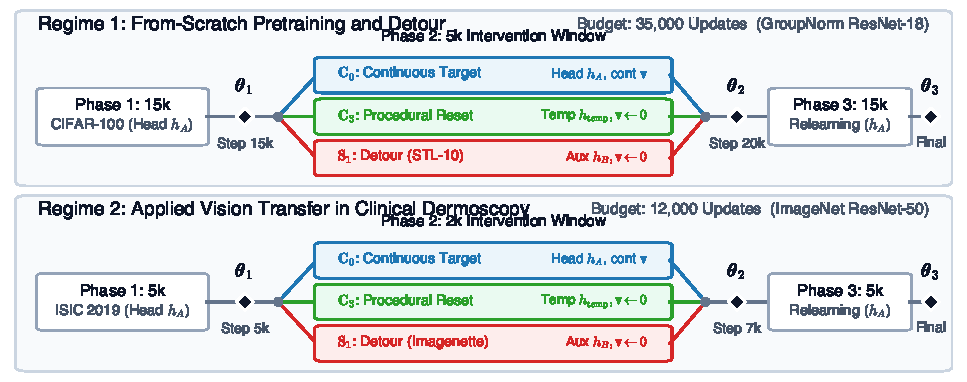
\includegraphics[width=\textwidth]{figures/figure_edafnet_style_framework.pdf}
\caption{\textbf{Overview of the controlled training schedules and evaluation protocol.} Three-phase schedule comparing continuous target training ($C_0$), on-target procedural reset control ($C_3$), and auxiliary detour ($S_1$) on CIFAR-100 and STL-10 under an equal total budget of 35k updates. Terminal test accuracies are evaluated across $N = 20$ paired random seeds (mean $\pm$ SD; Table~\ref{tab:seed_level_results}). Longitudinal representation metrics (frozen linear probe accuracy and Effective Rank) are evaluated across the $N = 6$ paired cohort at steps 15k, 20k, and 35k (Table~\ref{tab:representation_trajectories}), supporting confirmatory evaluation of Hypotheses H1, H2, and RQ3.}\label{fig:framework_architecture}\label{fig:method_schematic}
\end{figure*}

\begin{table*}[t]
\caption{Detailed intervention, exposure, and state matrix for all experimental arms evaluated in the confirmatory study. All arms utilize a GroupNorm ResNet-18 backbone with constant learning rate $\eta = 0.1$.}\label{tab:intervention_matrix}
\centering
\resizebox{0.88\textwidth}{!}{%
\begin{tabular}{llp{2.5cm}cccc}
\toprule
\textbf{Arm / Milestone} & \textbf{Phase 2 Data} & \textbf{Phase 2 Head} & \textbf{Resets} & \textbf{Target Updates} & \textbf{Aux Updates} & \textbf{Total Updates} \\
\midrule
$C_0$ (30k Comparator) & CIFAR-100 & Target $h_A$ & None & 30k & 0 & 30k \\
$C_0$ (35k Terminal)   & CIFAR-100 & Target $h_A$ & None & 35k & 0 & 35k \\
$C_3$ (35k Terminal)   & CIFAR-100 & Temp $h_{\mathrm{temp}}$ (100 cls) & 15k, 20k & 35k & 0 & 35k \\
$S_1$ (35k Terminal)   & STL-10    & Aux $h_B$ (10 cls) & 15k, 20k & 30k & 5k & 35k \\
\bottomrule
\end{tabular}%
}
\end{table*}

\subsection{State Management and Boundary Transition Rules}\label{subsec:schedule_transitions}

Four state rules govern the milestone transitions at 15,000 and 20,000 updates:
\paragraph{Backbone Parameter Continuity:} Feature backbone weights $\bm{\theta}_{\mathrm{bb}}$ track an unbroken trajectory across all phases without reinitialization: $\bm{\theta}_{\mathrm{bb}}^{(t)} = \bm{\theta}_{\mathrm{bb}}^{(t-1)} - \eta \, \bm{v}_{\mathrm{bb}}^{(t)}$.
\paragraph{Classification Head Preservation and Restoration:} For arms $C_3$ and $S_1$, head weights $\bm{w}_A^{(1)}$ at step $15{,}000$ are cached in host memory during Phase~2. At step $20{,}000$, we discard the Phase~2 classification head and re-attach $\bm{w}_A^{(1)}$, recovering the exact pre-intervention projection.
\paragraph{Optimizer Momentum Resets:} SGD operates with momentum parameter $\mu = 0.9$ and learning rate $\eta = 0.1$, stepping velocity via $\bm{v}_t = \mu \, \bm{v}_{t-1} + \nabla_{\!\bm{\theta}} \mathcal{L}(\bm{\theta}_{t-1}; \mathcal{B}_t)$. Under $C_0$, $\bm{v}_t$ carries forward continuously. Under $C_3$ and $S_1$, we zero the backbone velocity vectors ($\bm{v}_{\mathrm{bb}} \leftarrow \mathbf{0}$) at both boundaries ($t = 15{,}000$ and $t = 20{,}000$).
\paragraph{Normalization Invariance (Group Normalization):} Standard Batch Normalization tracks mini-batch running statistics that drift when models alternate between disparate datasets. To prevent this covariate shift, the backbone relies entirely on Group Normalization ($G = 32$ groups) \cite{wu2018groupnorm}. GroupNorm calculates statistics per instance across channel groups, ensuring activations remain sample-independent without cross-dataset running-mean distortion.

Table~\ref{tab:intervention_matrix} details dataset exposure, classifier head assignments, momentum reset points, and update allocations across every evaluated arm.

\subsection{Formal Specification of Comparative Estimands}\label{subsec:schedule_estimands}

We define four paired contrasts to adjudicate computational, exposure, procedural, and transfer effects:
\begin{align}
    \Delta_{\mathrm{total}} &\triangleq \mathrm{Acc}(S_1; 35\,\mathrm{k}) - \mathrm{Acc}(C_0; 35\,\mathrm{k}), \label{eq:delta_total} \\
    \Delta_{\mathrm{target}} &\triangleq \mathrm{Acc}(S_1; 35\,\mathrm{k}) - \mathrm{Acc}(C_0; 30\,\mathrm{k}), \label{eq:delta_target} \\
    \Delta_{\mathrm{proc}} &\triangleq \mathrm{Acc}(C_3; 35\,\mathrm{k}) - \mathrm{Acc}(C_0; 35\,\mathrm{k}), \label{eq:delta_proc} \\
    \Delta_{\mathrm{aux}} &\triangleq \mathrm{Acc}(S_1; 35\,\mathrm{k}) - \mathrm{Acc}(C_3; 35\,\mathrm{k}). \label{eq:delta_aux}
\end{align}
\paragraph{Equal Total Updates ($\Delta_{\mathrm{total}}$):} Evaluates Hypothesis H1 under a matched computational ceiling. Both $S_1$ and $C_0$ consume 35,000 updates, but $S_1$ trades 5,000 target updates for auxiliary STL-10 steps.
\paragraph{Equal Target Exposure ($\Delta_{\mathrm{target}}$):} Tests whether auxiliary learning provides supplementary transfer beyond target training, comparing $S_1$ (30k target updates) against $C_0$ at step 30,000.
\paragraph{Procedural Reset Impact ($\Delta_{\mathrm{proc}}$):} Evaluates Hypothesis H2 by measuring the net effect of head substitution and momentum clearing on CIFAR-100 without auxiliary data.
\paragraph{Auxiliary Data Contribution ($\Delta_{\mathrm{aux}}$):} Measures the marginal difference between auxiliary STL-10 data and target CIFAR-100 data under matched boundary operations.

\subsection{Mechanistic \texorpdfstring{$2 \times 2$}{2x2} Factorial Decomposition Protocol}\label{subsec:schedule_factorial}

Control arm $C_3$ resets both the classification head and optimizer momentum simultaneously. To isolate their individual contributions, we run a $2 \times 2$ factorial experiment on CIFAR-100 across 35,000 updates, manipulating two binary treatment factors at steps $15{,}000$ and $20{,}000$:
\begin{itemize}
\item \textbf{Head Substitution ($h \in \{0, 1\}$):} At $h = 0$, target head $h_A$ remains attached throughout; at $h = 1$, we stash $h_A$ at step $15{,}000$, train on a temporary head $h_{\mathrm{temp}}$ during Phase~2, and re-attach $h_A$ at step $20{,}000$.
\item \textbf{Momentum Reset ($m \in \{0, 1\}$):} At $m = 0$, velocity vectors $\bm{v}_{\mathrm{bb}}$ carry over across phases; at $m = 1$, we zero the velocity buffers ($\bm{v}_{\mathrm{bb}} \leftarrow \mathbf{0}$) at each boundary.
\end{itemize}

This design defines four arms: $F_{00}$ (Continuous Baseline $C_0$), $F_{01}$ (Momentum Flush Only), $F_{10}$ (Head Substitution Only), and $F_{11}$ (Bundled Reset Control $C_3$). With $\mu_{hm}$ denoting mean test accuracy under condition $(h, m)$, we calculate main effects and interaction as:
\begin{align}
    \Delta_{\mathrm{head}} &\triangleq \frac{1}{2} \left[ (\mu_{10} - \mu_{00}) + (\mu_{11} - \mu_{01}) \right], \label{eq:factorial_head} \\
    \Delta_{\mathrm{mom}}  &\triangleq \frac{1}{2} \left[ (\mu_{01} - \mu_{00}) + (\mu_{11} - \mu_{10}) \right], \label{eq:factorial_mom} \\
    \Delta_{\mathrm{interaction}} &\triangleq (\mu_{11} - \mu_{01}) - (\mu_{10} - \mu_{00}). \label{eq:factorial_interaction}
\end{align}
All conditions within a seed block fork from the common checkpoint $\bm{\theta}_1$, preserving repeated-measures pairing across seeds.

\section{Experimental Setup and Analysis Protocol}\label{sec:protocol}

\subsection{Datasets, Preprocessing, and Split Partitions}\label{subsec:protocol_datasets}

We evaluate multi-phase schedules on two standard computer vision benchmarks: CIFAR-100 \cite{krizhevsky2009cifar} as the target task and STL-10 \cite{coates2011stl10} as the auxiliary detour.

Target classification uses CIFAR-100 (60{,}000 $32 \times 32$ images across 100 classes). We enforce strict split quarantine. The 50{,}000 training examples are partitioned into 45{,}000 images for backbone parameter optimization and linear probe fitting, and a 5{,}000-image validation split reserved strictly for out-of-sample probe evaluation and hyperparameter auditing. The 10{,}000-image test set remains completely quarantined; test labels are touched only once at terminal schedule endpoints ($t = 30{,}000$ and $35{,}000$). For intermediate geometric diagnostics, we pass a fixed subset of 2{,}000 unlabeled inputs without label access.

The auxiliary domain, STL-10, provides 5{,}000 labeled images over 10 object classes. To match the spatial resolution of the CIFAR-100 trunk, native $96 \times 96$ images are downsampled to $32 \times 32$ pixels via bicubic anti-aliased interpolation. Both tasks share identical training data augmentation: random horizontal flips ($p = 0.5$) and random crops to $32 \times 32$ from inputs padded with 4 border pixels, followed by standard per-channel normalization.

\subsection{Network Architecture and Optimization Hyperparameters}\label{subsec:protocol_model}

All experiments instantiate a modified ResNet-18 backbone \cite{he2016deep} adapted for $32 \times 32$ inputs.

Standard Batch Normalization introduces running mean and variance buffers that drift unpredictably when switching between disparate task distributions. We eliminate this confound entirely by replacing all normalization layers with Group Normalization ($G = 32$ groups) \cite{wu2018groupnorm}. GroupNorm computes statistics independently per instance across channel groups. Activations thus remain strictly batch-independent and immune to running covariate shift.

Adaptive average pooling condenses backbone features into a penultimate embedding $\bm{z} \in \mathbb{R}^{512}$. Classification heads attach directly to $\bm{z}$ as single linear transformations ($\bm{W}\bm{z} + \bm{b}$), projecting to $K = 100$ logits for CIFAR-100 or $K = 10$ logits for STL-10. Optimization uses mini-batch SGD with momentum $\mu = 0.9$, weight decay $5 \times 10^{-4}$, and mini-batch size $B = 128$. Most importantly, the learning rate remains constant at $\eta = 0.1$ across the entire 35{,}000-update budget. We deliberately avoid learning rate annealing: decaying step sizes would introduce temporal non-stationarity, masking whether accuracy shifts stem from schedule structure or learning rate decay.

\subsection{Diagnostic Representation Metrics}\label{subsec:protocol_diagnostics}

Downstream classifier accuracy captures only the final mapping from logits to labels. To inspect internal feature organization without confounding from readout weights, we audit representations at three critical milestones: pre-interruption ($t = 15{,}000$), post-interruption ($t = 20{,}000$), and relearning completion ($t = 35{,}000$).

\subsubsection{Matched Frozen Linear Probes}\label{subsubsec:protocol_probes}
Linear classifier probes measure the accessibility of target classes independently of the active network head \cite{alain2017understanding,davari2022probing}. At each milestone checkpoint $\bm{\theta}_{\mathrm{bb}}$, we lock backbone weights under \texttt{torch.no\_grad()} and extract 512-dimensional penultimate embeddings for the 45{,}000 training and 5{,}000 validation images. On an isolated copy of the model with a dedicated random seed, we train a linear probe ($\bm{W}_{\mathrm{probe}} \in \mathbb{R}^{100 \times 512}, \bm{b}_{\mathrm{probe}} \in \mathbb{R}^{100}$) on the 45{,}000 training representations for 5 epochs using Adam ($\eta = 10^{-3}$, weight decay $10^{-4}$, batch size 128) under multi-class cross-entropy loss.

Probe performance is recorded strictly on the held-out 5{,}000-example validation split. This out-of-sample protocol prevents label leakage and guarantees that test partitions remain untouched. Crucially, linear probing decouples classifier head disruption from backbone degradation. When a head is swapped or its gradients fluctuate, test accuracy drops; probing reveals whether target class boundaries remain linearly separable in the latent geometry. Probing is an accessibility check, however, not proof of metric invariance. High probe accuracy confirms linear separability, but cannot detect coordinate shears, isotropic expansion, or rotations within the feature space.

\subsubsection{Effective Rank}\label{subsubsec:protocol_rank}
To detect feature collapse and track geometric dimensionality, we evaluate Effective Rank ($\EffRank$) \cite{roy2007effective,begga2026preserving}. Let $\bm{Z}_{\mathrm{raw}} \in \mathbb{R}^{N \times d}$ denote penultimate features extracted under \texttt{torch.no\_grad()} for $N = 2{,}000$ unlabeled test examples, and let $\bm{Z} = (\bm{I}_N - \frac{1}{N}\bm{1}\bm{1}^\top)\bm{Z}_{\mathrm{raw}}$ be the centered feature matrix. For singular values $\sigma_1 \ge \dots \ge \sigma_r > 0$ with $r = \min(N, d) = 512$, the normalized singular value spectrum $p_k = \sigma_k / \sum_{j=1}^r \sigma_j$ forms a probability distribution. Effective Rank exponentiates the Shannon entropy of this spectrum:
\begin{equation}\label{eq:effrank}
    \EffRank(\bm{Z}) \triangleq \exp(H(\bm{Z})) = \exp\left( -\sum_{k=1}^r p_k \ln p_k \right).
\end{equation}
The metric spans $[1, 512]$ on the coordinate scale. An $\EffRank$ of 1 denotes complete dimensional collapse onto a single eigenvector. An $\EffRank$ of 512 represents a perfectly spherical, isotropic feature distribution.

\subsubsection{Linear Centered Kernel Alignment and Representational Drift}\label{subsubsec:protocol_cka}
Centered Kernel Alignment (CKA) compares pairwise similarity geometry across checkpoints without enforcing coordinate alignment \cite{kornblith2019similarity}. For centered penultimate feature matrices $\bm{Z}_{\mathrm{pre}}, \bm{Z}_t \in \mathbb{R}^{N \times d}$ computed on the identical $N = 2{,}000$ unlabeled inputs at step $15{,}000$ and step $t$, linear CKA normalizes the Frobenius inner product of their Gram matrices:
\begin{equation}
    \mathrm{CKA}(\bm{Z}_{\mathrm{pre}}, \bm{Z}_t) \triangleq \frac{\|\bm{Z}_t^\top \bm{Z}_{\mathrm{pre}}\|_F^2}{\|\bm{Z}_{\mathrm{pre}}^\top \bm{Z}_{\mathrm{pre}}\|_F \, \|\bm{Z}_t^\top \bm{Z}_t\|_F}.
\end{equation}
Because linear CKA remains invariant to orthogonal rotations and uniform scaling, we measure representational drift via its complement:
\begin{equation}\label{eq:dcka}
    \Dcka \triangleq 1 - \mathrm{CKA}(\bm{Z}_{\mathrm{pre}}, \bm{Z}_t) \in [0, 1],
\end{equation}
where $\Dcka = 0$ indicates identical similarity structure and $\Dcka \to 1$ indicates complete geometric divergence. Pairing $\Dcka$ with Effective Rank separates rigid feature space rotation from subspace volume collapse.

\subsubsection{Target Recovery Latency}\label{subsubsec:protocol_urec}
Target recovery latency tracks how many Phase-3 updates elapse before validation accuracy regains its pre-interruption baseline performance:
\begin{equation}\label{eq:urec}
    \urec \triangleq \min \{ u \ge 0 : \mathrm{Acc}(\bm{\theta}_{20\mathrm{k} + u}) \ge \mathrm{Acc}(\bm{\theta}_{15\mathrm{k}}) \}.
\end{equation}
We evaluate target validation accuracy at 100-update increments throughout Phase 3 ($u \in \{0, 100, \dots, 15{,}000\}$). If accuracy meets or exceeds the baseline at the initial return step ($t = 20{,}000$), $\urec = 0$. If a run fails to recover baseline performance before the update budget expires, it is right-censored at $\urec > 15{,}000$.

\subsection{Prespecified Paired Statistical Analysis Protocol}\label{subsec:protocol_statistics}

All inferential procedures were prespecified and locked prior to executing confirmatory trials.

\paragraph{Paired Seed Design, Chronology, and Sensitivity Partition:}
Data collection followed a two-stage protocol. We first ran an exploratory cohort of six paired seeds ($s \in \{920001, \dots, 920006\}$) to calibrate baseline variances and verify the $2 \times 2$ factorial decomposition. Once complete, we froze the entire experimental protocol without alteration: network architecture (GroupNorm ResNet-18), optimization parameters ($\eta = 0.1$, batch size 128, momentum 0.9), schedule transitions ($15\,\mathrm{k}, 20\,\mathrm{k}, 35\,\mathrm{k}$ updates), boundary reset rules, checkpoint branching from $\bm{\theta}_1^{(s)}$, and the primary estimand ($S_1 - C_0$). To reduce margin of error below $\pm 0.6$ pp, we prospectively enrolled fourteen additional paired seeds ($s \in \{920007, \dots, 920020\}$), bringing the sample to $N = 20$. To guarantee that exploratory observations do not bias final inferences, we evaluate an independent sensitivity partition separating the six initial seeds from the fourteen prospective confirmatory seeds.

\paragraph{Primary Paired Inferential Test:}
Let $d_s = \mathrm{Acc}(S_1; s) - \mathrm{Acc}(C_0; s)$ denote the paired difference in terminal test accuracy for seed $s$ under 35,000 updates. The primary test of Hypothesis H1 is a two-sided paired Student's $t$-test on $\{d_s\}_{s=1}^N$ with $N-1$ degrees of freedom. We report the sample mean difference $\bar{d}$, paired standard deviation $s_d$, standard error $\mathrm{SE} = s_d / \sqrt{N}$, test statistic $t = \bar{d} / \mathrm{SE}$, two-sided $p$-value, and the parametric $95\%$ paired $t$-interval $\bar{d} \pm t_{0.975, N-1} \cdot \mathrm{SE}$ ($t_{0.975, 19} = 2.093$ for $N = 20$; $t_{0.975, 9} = 2.262$ for $N = 10$).

\paragraph{Non-Parametric Bootstrap and Permutation Benchmarks:}
We cross-check parametric tests against non-parametric alternatives: $10{,}000$-iteration percentile bootstrap intervals and exact sign-flip permutation tests (evaluating all $2^{20} = 1{,}048{,}576$ sign combinations at $N = 20$). Because percentile bootstrap intervals resample the discrete empirical differences without assuming normality, they reflect sample skewness. In smaller cohorts ($N = 10$ archival runs), empirical percentile intervals diverge slightly from symmetric $t$-intervals due to sample asymmetry (e.g., archival contrast $B_4 - B_1$, paired $t$-interval [$-1.74$, $+0.68$] pp vs.\ bootstrap [$-1.48$, $+0.52$] pp). We explicitly distinguish intervals throughout all tables and text as either parametric Student's $t$-intervals (\texttt{Paired $t$-CI}) or empirical percentile bootstrap intervals (\texttt{Boot CI}).

\paragraph{Discrepancy Adjudication Rule and Multiplicity Control:}
We designate the parametric paired Student's $t$-test as the binding confirmatory decision rule. When the primary test fails to reject the null at $\alpha = 0.05$, a bootstrap interval whose boundary marginally excludes zero due to small-sample skewness cannot override the parametric decision. Confirmatory error protection is reserved for the primary contrast ($S_1 - C_0$). Secondary contrasts ($S_1 - C_3$, $C_3 - C_0$, and $S_1 - C_0(30\mathrm{k})$) are evaluated under Bonferroni correction at $\alpha_{\mathrm{adj}} = 0.05 / 3 \approx 0.0167$. For CViT evaluations, the Bonferroni threshold is $\alpha_{\mathrm{adj}} = 0.05 / 2 = 0.025$.

\paragraph{Statistical Precision and Minimum Detectable Effect:}
Under $N = 20$ paired seeds, two-sided $\alpha = 0.05$, and observed sample standard deviation $s_d = 1.0822$ pp, the empirical standard error is $\mathrm{SE} = 0.2420$ pp, yielding a margin of error of $\pm 0.51$ pp. At $80\%$ statistical power ($\beta = 0.20$, two-sided paired $t$-test, critical effect size $d_z = 0.660$), this design guarantees sensitivity down to a minimum detectable effect of $\mathrm{MDE} = 0.71$ pp. This boundary confirms that the study is sufficiently powered to detect shifts exceeding three-quarters of a percentage point, defining the resolution limit of our negative finding.

\section{Empirical Results}\label{sec:results}

\subsection{Primary Confirmatory Evaluation: Resolving Hypothesis H1}\label{subsec:results_primary}

Our primary hypothesis (H1) asserts that inserting an intermediate off-task training detour ($S_1$) improves terminal CIFAR-100 test accuracy over uninterrupted continuous optimization ($C_0$) under a fixed compute ceiling of 35,000 updates ($\Delta_{\mathrm{total}} > 0$).

The paired twenty-seed evaluation refutes this claim. Across seeds 920001--920020, continuous training reaches $56.69\%$ mean test accuracy ($s = 0.75\%$), whereas the auxiliary detour attains $56.26\%$ ($s = 1.51\%$). As shown in Table~\ref{tab:inferential_statistics} and Figure~\ref{fig:paired_contrasts_forest}, the sample mean paired contrast is negative:
\begin{equation}
    \bar{d}_{\mathrm{total}} = -0.4325 \text{ percentage points (pp)},
\end{equation}
with sample standard deviation $s_d = 1.0822$ pp and standard error $\mathrm{SE} = 0.2420$ pp.

\begin{figure*}[t]
\centering
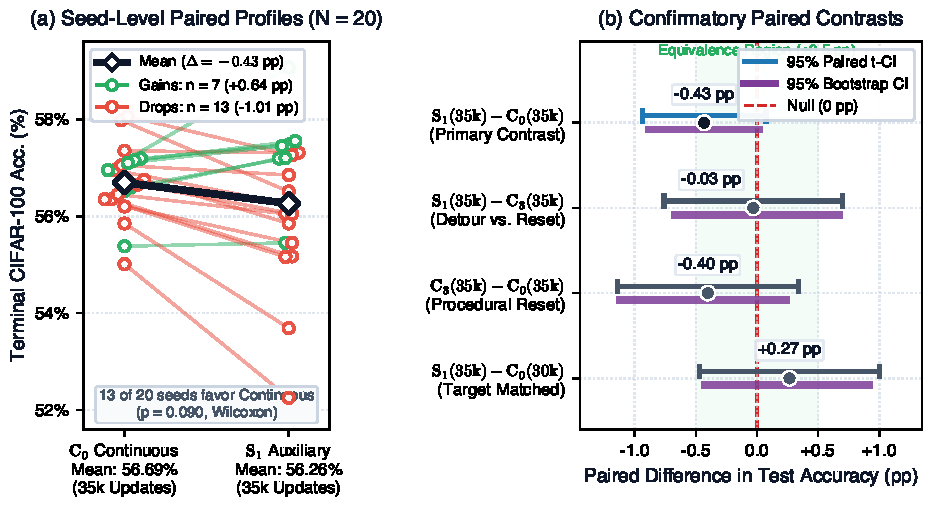
\includegraphics[width=0.84\textwidth]{figures/figure_paired_contrasts_forest_plot.pdf}
\caption{Confirmatory and secondary paired contrast inferential analysis across $N = 20$ matched seeds: (a) Seed-level paired slope trajectories from $C_0(35\mathrm{k})$ to $S_1(35\mathrm{k})$ ($\bar{d}_{\mathrm{total}} = -0.43$ pp); (b) Confirmatory forest plot showing point estimates, parametric $95\%$ Student's $t$-intervals, and non-parametric $95\%$ bootstrap intervals; (c) Exact sign-flip permutation null distribution across all $2^{20} = 1{,}048{,}576$ sign configurations ($p_{\mathrm{perm}} = 0.0906$).}\label{fig:paired_contrasts_forest}
\end{figure*}

\begin{table*}[t]
\caption{Confirmatory inferential statistics for primary and secondary schedule contrasts across $N = 20$ paired seeds. Contrasts are expressed in percentage points (pp).}\label{tab:inferential_statistics}
\centering
\renewcommand{\arraystretch}{0.9}
\resizebox{0.92\textwidth}{!}{%
\begin{tabular}{lcccccc}
\toprule
\textbf{Contrast Estimand} & \textbf{Mean Diff.} & \textbf{Paired SD} & \textbf{95\% Paired $t$-CI} & \textbf{$t$-statistic} & \textbf{$p$-value} & \textbf{95\% Bootstrap CI} \\
\midrule
\textbf{Primary:} $S_1(35\mathrm{k}) - C_0(35\mathrm{k})$ & $\bm{-0.43}$ & 1.08 & [$-0.94$, $+0.07$] & $-1.79$ & 0.090 & [$-0.89$, $+0.02$] \\
Secondary: $S_1(35\mathrm{k}) - C_3(35\mathrm{k})$        & $-0.03$      & 1.56 & [$-0.76$, $+0.70$] & $-0.09$ & 0.933 & [$-0.67$, $+0.67$] \\
Secondary: $C_3(35\mathrm{k}) - C_0(35\mathrm{k})$        & $-0.40$      & 1.58 & [$-1.14$, $+0.34$] & $-1.14$ & 0.269 & [$-1.12$, $+0.24$] \\
Secondary: $S_1(35\mathrm{k}) - C_0(30\mathrm{k})$        & $+0.27$      & 1.57 & [$-0.47$, $+1.00$] & $+0.76$ & 0.458 & [$-0.43$, $+0.92$] \\
\bottomrule
\end{tabular}%
}
\end{table*}

A two-sided paired Student's $t$-test yields $t(19) = -1.7873, p = 0.0898$ (parametric $95\%$ CI: [$-0.9390$, $+0.0740$] pp). Non-parametric checks corroborate this result: the $10{,}000$-iteration bootstrap interval covers [$-0.8880$, $+0.0200$] pp, and exact sign-flip permutation gives $p_{\mathrm{perm}} = 0.0906$. At the seed level, thirteen of twenty runs favor continuous training (deficits ranging from $-0.04$ to $-2.76$ pp), whereas only seven favor the detour (+0.07 to +2.12 pp). With $p > 0.05$ and a negative point estimate ($\bar{d} = -0.43$ pp), \textbf{the data fail to support Hypothesis H1}. Diverting compute to STL-10 yields no terminal benefit.

\paragraph{Cohort Partition Sensitivity Check:}
To verify that pooling across stages does not distort conclusions, we partition the twenty seeds into exploratory and prospective cohorts. The exploratory group ($N = 6$, seeds 920001--920006) yields $\bar{d} = -0.8933$ pp ($s_d = 1.4278$ pp, $t(5) = -1.53, p = 0.1860, 95\%$ CI: [$-2.39$, $+0.61$] pp). The prospective cohort gathered after protocol freezing ($N = 14$, seeds 920007--920020) likewise remains negative at $\bar{d} = -0.2350$ pp ($s_d = 0.8874$ pp, $t(13) = -0.99, p = 0.3398, 95\%$ CI: [$-0.75$, $+0.28$] pp), with ten of fourteen seeds showing non-positive differences ($d_s \le 0$). The lack of auxiliary advantage is consistent across both sub-cohorts.

\subsection{Secondary Schedule Contrasts}\label{subsec:results_secondary}

\subsubsection{Auxiliary STL-10 Data vs.\ On-Target Reset Control (\texorpdfstring{$\Delta_{\mathrm{aux}}$}{Delta-aux})}
Contrasting $S_1$ directly with $C_3$ tests the effect of substituting 5,000 auxiliary STL-10 gradient updates for 5,000 target CIFAR-100 updates while holding boundary resets identical. Across twenty paired seeds, the mean difference is negligible: $-0.0300$ pp ($s_d = 1.5632$ pp, $t(19) = -0.0858, p = 0.9325, p_{\mathrm{perm}} = 0.9336$), with a $95\%$ paired $t$-interval of [$-0.76$, $+0.70$] pp. Replacing target batches with auxiliary images provides no measurable transfer advantage. We note, however, that $S_1$ and $C_3$ differ along multiple dimensions simultaneously (task distribution, class semantics, and loss landscape), so this contrast estimates the compound package difference rather than isolated semantic transfer.

\subsubsection{Equal Target Exposure Budget (\texorpdfstring{$\Delta_{\mathrm{target}}$}{Delta-target})}
Comparing $S_1(35\mathrm{k})$ against $C_0(30\mathrm{k})$ equates target task exposure at 30,000 updates, granting $S_1$ 5,000 bonus STL-10 steps. Checkpoint $C_0(30\mathrm{k})$ reaches $56.00\%$ ($s = 0.48\%$). The resulting paired contrast is $+0.2660$ pp ($s_d = 1.5705$ pp, $t(19) = 0.7575, p = 0.4581, p_{\mathrm{perm}} = 0.4633, 95\%$ CI: [$-0.47$, $+1.00$] pp). Even when given 5,000 additional gradient steps beyond target baseline compute, the auxiliary schedule achieves no statistically detectable improvement.

\subsection{Procedural Reset Impact and \texorpdfstring{$2 \times 2$}{2x2} Factorial Decomposition: Evaluating Hypothesis H2}\label{subsec:results_procedural}

Hypothesis H2 posits that boundary procedural operations (swapping heads and zeroing momentum) do not systematically alter terminal accuracy on the primary task ($\Delta_{\mathrm{proc}} = 0$).

Comparing bundled control $C_3$ with continuous training $C_0$ across all twenty seeds at step 35,000 yields an observed difference of $-0.4025$ pp ($s_d = 1.5807$ pp, $t(19) = -1.1388, p = 0.2690, p_{\mathrm{perm}} = 0.2751, 95\%$ CI: [$-1.14$, $+0.34$] pp). Because the estimation interval easily spans zero, \textbf{the twenty-seed data fail to reject the null hypothesis of bundled procedural invariance ($\Delta_{\mathrm{proc}} = 0$)}. At the aggregate package level, procedural interventions produce no statistically reliable net shift.

Yet aggregate neutrality masks strong opposing forces. Our $2 \times 2$ factorial experiment on CIFAR-100 ($N = 6$ paired seeds; Table~\ref{tab:factorial_decomposition}) demonstrates that individual procedural components exert active, cancelling effects:

\begin{table*}[t]
\caption{Empirical $2 \times 2$ factorial decomposition of procedural interventions on CIFAR-100 under equal total budget ($35{,}000$ updates across $N = 6$ paired seeds). Accuracies are mean percentages $\pm$ standard deviation; contrasts $\Delta$ denote paired differences relative to baseline $F_{00}$ ($C_0$). $95\%$ CIs denote paired Student's $t$-intervals ($5$ d.f.); $p$-values are two-sided. Individual seed-level metrics are cataloged in Appendix~\ref{sec:appendix_factorial}.}\label{tab:factorial_decomposition}
\centering
\resizebox{0.92\textwidth}{!}{%
\begin{tabular}{llccccc}
\toprule
\textbf{Arm} & \textbf{Head Policy ($h$)} & \textbf{Momentum Policy ($m$)} & \textbf{Mean Acc. (\%)} & $\bm{\Delta}$ \textbf{vs.} $\bm{F_{00}}$ \textbf{(pp)} & \textbf{95\% CI} & $\bm{p}$ \\
\midrule
$F_{00}$ ($C_0$) & Retained target $h_A$ & Continuous carryover & $56.32 \pm 1.13$ & \textemdash & \textemdash & \textemdash \\
$F_{01}$         & Retained target $h_A$ & Zeroed ($\bm{v} \leftarrow \mathbf{0}$) & $56.88 \pm 0.86$ & $+0.56$ & [$-0.53$, $+1.65$] & $0.246$ \\
$F_{10}$         & Temp head $h_{\mathrm{temp}}$ & Continuous carryover & $54.21 \pm 1.21$ & $-2.11$ & [$-3.40$, $-0.83$] & $0.008$ \\
$F_{11}$ ($C_3$) & Temp head $h_{\mathrm{temp}}$ & Zeroed ($\bm{v} \leftarrow \mathbf{0}$) & $54.79 \pm 1.32$ & $-1.53$ & [$-3.73$, $+0.67$] & $0.133$ \\
\midrule
\multicolumn{7}{l}{\textit{Factorial Main Effects and Interaction Contrast:}} \\
\multicolumn{3}{l}{Main effect of head substitution ($\Delta_{\mathrm{head}}$)} & \multicolumn{2}{c}{$-2.10$ pp} & [$-3.18$, $-1.02$] & $0.004$ \\
\multicolumn{3}{l}{Main effect of momentum clearing ($\Delta_{\mathrm{mom}}$)}   & \multicolumn{2}{c}{$+0.57$ pp} & [$-0.64$, $+1.77$] & $0.279$ \\
\multicolumn{3}{l}{Factorial interaction ($\Delta_{\mathrm{interaction}}$)}      & \multicolumn{2}{c}{$+0.02$ pp} & [$-1.25$, $+1.29$] & $0.967$ \\
\bottomrule
\end{tabular}%
}
\end{table*}

\paragraph{Head Substitution Penalty ($\Delta_{\mathrm{head}} = -2.10$ pp, $p = 0.004$):}
Swapping the classifier head while maintaining momentum ($F_{10}$) incurs a significant $-2.11$ pp penalty relative to uninterrupted training ($95\%$ CI: [$-3.40$, $-0.83$] pp, $p = 0.008$). Across both momentum levels, the marginal main effect of head replacement is $\Delta_{\mathrm{head}} = -2.10$ pp ($95\%$ CI: [$-3.18$, $-1.02$] pp, two-way repeated-measures ANOVA $F(1, 5) = 24.95, p = 0.004$). Reinitializing the output layer abruptly reshapes backpropagated gradient variance into the shared backbone \cite{lapacz2025exploring}, inflicting a clear performance cost.

\paragraph{Momentum Buffer Reset ($\Delta_{\mathrm{mom}} = +0.57$ pp, $p = 0.279$):}
Conversely, zeroing momentum buffers ($\bm{v} \leftarrow \mathbf{0}$) shifts accuracy upward by $+0.57$ pp, though with high estimation variance ($95\%$ CI: [$-0.64$, $+1.77$] pp, $F(1, 5) = 1.47, p = 0.279$). In isolation ($F_{01}$ vs.\ $F_{00}$), clearing momentum reaches $56.88\%$ (+0.56 pp, $95\%$ CI: [$-0.53$, $+1.65$] pp, $p = 0.246$). Alongside head replacement ($F_{11}$ vs.\ $F_{10}$), it yields $54.79\%$ vs.\ $54.21\%$ (+0.58 pp). The interaction between the two factors is strictly additive ($\Delta_{\mathrm{interaction}} = +0.02$ pp, $95\%$ CI: [$-1.25$, $+1.29$] pp, $F(1, 5) = 0.002, p = 0.967$). While the positive point estimate suggests that flushing stale velocity vectors might relieve optimization hysteresis, the confidence interval spans zero, so this effect remains statistically unconfirmed.

\paragraph{Decoupling Factorial Components from Bundled Outcomes (Hypothesis H2):}
The six-seed factorial analysis and the twenty-seed confirmatory study answer different questions. In the factorial cohort, the opposing effects cancel out ($-2.10 + 0.57 = -1.53$ pp, matching $F_{11} - F_{00} = -1.53$ pp, $p = 0.133$). But this decomposition cannot be used to reject procedural invariance in the larger confirmatory cohort, where bundled control $C_3$ remains statistically indistinguishable from baseline $C_0$ ($-0.4025$ pp, $p = 0.2690$). Procedural resets cannot be dismissed as harmless overhead, nor can momentum clearing be assumed to compensate reliably for head substitution in wider populations.

\subsection{Longitudinal Representation Trajectory Dynamics}\label{subsec:results_representations}

Downstream test metrics track final classification outcomes, but conceal internal representational transitions. To trace how latent manifolds evolve during off-task detours (RQ3), we audit frozen linear decodability and Effective Rank across milestone checkpoints ($15\,\mathrm{k}, 20\,\mathrm{k}, 35\,\mathrm{k}$).

\begin{table*}[t]
\caption{Longitudinal representation diagnostics at key milestones: Step 15,000 (pre-interruption checkpoint $\theta_1$), Step 20,000 (post-interruption), and Step 35,000 (terminal relearning). Values denote mean (standard deviation) across six paired seeds.}\label{tab:representation_trajectories}
\centering
\resizebox{0.92\textwidth}{!}{%
\begin{tabular}{lcccccc}
\toprule
 & \multicolumn{3}{c}{\textbf{Matched Linear Probe Accuracy (\%)}} & \multicolumn{3}{c}{\textbf{Effective Rank ($\EffRank$)}} \\
\cmidrule(lr){2-4} \cmidrule(lr){5-7}
\textbf{Arm} & \textbf{Step 15k} & \textbf{Step 20k} & \textbf{Step 35k} & \textbf{Step 15k} & \textbf{Step 20k} & \textbf{Step 35k} \\
\midrule
Continuous Target ($C_0$)       & 60.07 (0.50) & 61.24 (0.59) & 63.01 (0.94) & 178.04 (7.85) & 171.21 (7.31) & 162.45 (6.69) \\
On-Target Reset Control ($C_3$) & 60.07 (0.50) & 61.03 (1.04) & 62.52 (1.08) & 178.04 (7.85) & 169.32 (6.98) & 162.37 (6.66) \\
Auxiliary Interval ($S_1$)      & 60.07 (0.50) & 20.65 (0.74) & 61.96 (0.85) & 178.04 (7.85) & 124.50 (5.52) & 153.69 (6.76) \\
\bottomrule
\end{tabular}%
}
\end{table*}

\begin{figure*}[t]
\centering
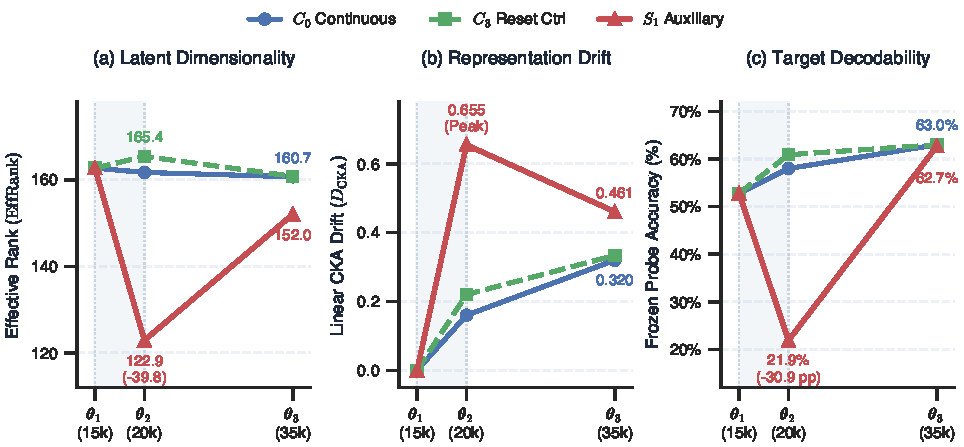
\includegraphics[width=0.85\textwidth]{figures/figure_longitudinal_representation_dynamics.pdf}
\caption{Longitudinal representation dynamics across training milestones ($15\mathrm{k}, 20\mathrm{k}, 35\mathrm{k}$ updates, evaluated at discrete checkpoints with visual interpolation lines; mean across $N = 6$ paired seeds): (a) Target decodability trajectory measured by matched frozen linear probe accuracy ($W_{\mathrm{probe}} \in \mathbb{R}^{100 \times 512}$), showing severe target amnesia during off-task learning ($20.65\%$) followed by rapid rebound to $61.96\%$ (vs.\ $C_0$ at $63.01\%$); (b) Geometric dimensionality measured by Effective Rank ($\EffRank(\bm{Z}) \in [1, 512]$), showing subspace entropy collapse ($\EffRank \to 124.50$) followed by re-expansion to $153.69$.}\label{fig:longitudinal_dynamics}
\end{figure*}

At step $15{,}000$ ($\bm{\theta}_1$), target representations attain a mean linear probe decodability of $60.07\%$ and an Effective Rank of $178.04$ across all arms. Phase 2 introduces severe divergence:
\paragraph{Acute Intermediate Collapse (Step 20,000):}
Off-task training on STL-10 ($S_1$) demolishes target decodability: probe accuracy drops by nearly 40 percentage points to $20.65\%$, while Effective Rank drops from $178.04$ to $124.50$, indicating severe subspace entropy compression \cite{begga2026preserving}. In contrast, on-target control $C_3$ advances smoothly to $61.03\%$ probe accuracy (matching continuous training $C_0$ at $61.24\%$) with Effective Rank held at $169.32$ (vs.\ $171.21$ in $C_0$). Procedural resets alone do not induce representational amnesia when training remains on-target.
\paragraph{Relearning Restitution (Step 35,000):}
Resuming CIFAR-100 training in Phase 3 triggers fast representational rebound: $S_1$ probe decodability surges from $20.65\%$ back to $61.96\%$, while Effective Rank re-expands to $153.69$. Yet this rebound remains incomplete. Continuous baseline $C_0$ reaches $63.01\%$ probe decodability and an Effective Rank of $162.45$.

These dynamics demonstrate that \textbf{internal representation recovery does not produce a downstream generalization advantage}. The network successfully restores linear separability (rebounding by $+41.31$ pp to $61.96\%$), yet its terminal test accuracy ($56.26\%$) lags continuous training ($56.69\%$; $-0.43$ pp, $p = 0.0898$). Internal manifold restitution is an insufficient condition for terminal performance gains.

\subsection{Mechanistic Sensitivity and Ablation Analyses}\label{subsec:results_ablations}

To evaluate boundary invariants and structural factors governing multi-phase schedules, we conduct exploratory ablations on GroupNorm ResNet-18 across three random seeds (seeds 42, 123, 456; Table~\ref{tab:ablation_summaries}).

\begin{table*}[t]
\caption{Mechanistic sensitivity and ablation summaries across $N = 3$ random seeds on GroupNorm ResNet-18. Accuracies are percentages (mean $\pm$ standard deviation); forgetting $F_B$ is expressed in percentage points (pp) and recovery time $u_{\mathrm{rec}}$ in optimizer updates.}\label{tab:ablation_summaries}
\centering
\resizebox{0.92\textwidth}{!}{%
\begin{tabular}{llccccc}
\toprule
\textbf{Ablation Axis} & \textbf{Intervention Configuration} & $N$ & \textbf{Final Val (\%)} & \textbf{Final Test (\%)} & \textbf{Forgetting $F_B$ (pp)} & \textbf{Recovery $u_{\mathrm{rec}}$} \\
\midrule
Timing ($35\mathrm{k}$ Budget) & Early ($u_1 = 5\mathrm{k}$, $25\mathrm{k}$ recovery)  & 3 & $56.31 \pm 1.61$ & --- & $33.01$ & $533.3$ \\
Timing ($35\mathrm{k}$ Budget) & Mid ($u_1 = 15\mathrm{k}$, $15\mathrm{k}$ recovery)    & 3 & $56.23 \pm 2.15$ & $56.95 \pm 2.02$ & $46.58$ & $2100.0$ \\
Timing ($35\mathrm{k}$ Budget) & Late ($u_1 = 25\mathrm{k}$, $5\mathrm{k}$ recovery)    & 3 & $56.05 \pm 2.03$ & --- & $47.39$ & $1766.7$ \\
Timing ($15\mathrm{k}$ Recovery) & Early ($u_1 = 5\mathrm{k}$, $25\mathrm{k}$ total)   & 3 & $54.45 \pm 1.66$ & --- & $33.01$ & $533.3$ \\
Timing ($15\mathrm{k}$ Recovery) & Late ($u_1 = 25\mathrm{k}$, $45\mathrm{k}$ total)    & 3 & $56.06 \pm 1.66$ & --- & $47.39$ & $1766.7$ \\
\midrule
Momentum ($S_1$, STL-10)       & Preserved (Backbone carryover)                       & 3 & $55.77 \pm 2.12$ & $56.37 \pm 1.31$ & $45.77$ & $2866.7$ \\
Momentum ($S_1$, STL-10)       & Zeroed (True zero reset, $\bm{v} \leftarrow \mathbf{0}$) & 3 & $\bm{56.91 \pm 0.53}$ & $\bm{57.13 \pm 0.17}$ & $46.26$ & $2766.7$ \\
Momentum ($C_3$, Reset)        & Preserved (Backbone carryover)                       & 3 & $55.35 \pm 0.82$ & $56.07 \pm 0.94$ & $-0.57$ & $133.3$ \\
Momentum ($C_3$, Reset)        & Zeroed (True zero reset, $\bm{v} \leftarrow \mathbf{0}$) & 3 & $\bm{57.31 \pm 0.25}$ & $\bm{57.55 \pm 0.52}$ & $-2.17$ & $266.7$ \\
\midrule
Replay Cushion                 & $90/10$ STL-10/CIFAR-100 Mixture                     & 3 & $55.34 \pm 2.79$ & $55.94 \pm 1.80$ & $\bm{16.65}$ & $\bm{1100.0}$ \\
Isolated Reference ($S_1$)     & $100\%$ STL-10 Interval                              & 3 & $56.23 \pm 2.15$ & $56.95 \pm 2.02$ & $46.58$ & $2100.0$ \\
\bottomrule
\end{tabular}%
}
\end{table*}

\subsubsection{Auxiliary Insertion Timing and Representational Vulnerability}
Under a fixed 35,000-update ceiling, earlier detours cause less representational amnesia. Interrupting training early ($u_1 = 5\,\mathrm{k}$, 25k recovery) incurs forgetting of $F_B = 33.01$ pp ($u_{\mathrm{rec}} = 533.3$ updates), whereas mid and late detours produce drops of $46.58$ pp and $47.39$ pp ($u_{\mathrm{rec}} = 2{,}100.0$ and $1{,}766.7$ updates). Specializing features are harder to disrupt than immature ones. Despite this fourfold divergence in recovery latency, terminal validation accuracy varies by less than $0.3$ pp across insertion points ($56.31\%$ early vs.\ $56.23\%$ mid vs.\ $56.05\%$ late).

\subsubsection{Optimizer Momentum Reset Dynamics}
In exploratory three-seed trials (Table~\ref{tab:ablation_summaries}), zeroing velocity buffers ($\bm{v} \leftarrow \mathbf{0}$) upon returning to the primary task produced sample test improvements of $+0.76$ pp in auxiliary schedule $S_1$ ($57.13\%$ vs.\ $56.37\%$) and $+1.48$ pp in reset control $C_3$ ($57.55\%$ vs.\ $56.07\%$). While this pilot signal suggests that clearing stale velocity vectors could relieve cross-task optimization drag, our six-seed factorial analysis on target data (Section~\ref{subsec:results_procedural}) demonstrated that the marginal momentum effect remains statistically uncertain ($\Delta_{\mathrm{mom}} = +0.57$ pp, $95\%$ CI: [$-0.64$, $+1.77$] pp, $p = 0.279$). Momentum clearing provides a favorable point estimate, not a confirmed generalizable buffer.

\subsubsection{Memory Replay Cushion Dynamics}
Interleaving a $10\%$ CIFAR-100 rehearsal stream during auxiliary training cushioned against catastrophic forgetting, reducing $F_B$ from $46.58$ pp to $16.65$ pp and halving recovery time from $2{,}100$ to $1{,}100$ updates. Yet representational preservation yielded zero generalization benefit: terminal test accuracy reached only $55.94\%$, trailing isolated auxiliary training at $56.95\%$ ($-1.01$ pp deficit).

\subsection{Architectural Generality: Compact Vision Transformers}\label{subsec:results_vit}

To verify whether representation recovery without generalization gains extends beyond convolutional networks, we replicate the schedule protocol on a Compact Vision Transformer (CViT; $4 \times 4$ patches, 6 layers, $D = 192$, 4 attention heads, $\approx 1.82\mathrm{M}$ parameters, LayerNorm, AdamW) across $N = 5$ paired seeds (seeds 3001--3005; Table~\ref{tab:vit_results}).

\begin{table*}[t]
\caption{Architectural generality evaluation on Compact Vision Transformers (CViT; $\approx 1.82\mathrm{M}$ parameters) across $N = 5$ seeds. Contrasts evaluate equal total budget ($\Delta_{\mathrm{total}} = 35\mathrm{k}$ updates) and equal target exposure ($\Delta_a = 30\mathrm{k}$ target updates). Primary CIs denote paired Student's $t$-intervals ($4$ d.f.); $p_{\mathrm{paired}}$ denotes two-sided paired Student's $t$-test; $d_z$ is paired Cohen's effect size.}\label{tab:vit_results}
\centering
\resizebox{\textwidth}{!}{%
\begin{tabular}{l c cccc cccc cc}
\toprule
& & \multicolumn{4}{c}{\textbf{Equal Total Updates ($\Delta_{\mathrm{total}}$, Val)}} & \multicolumn{4}{c}{\textbf{Equal Target Updates ($\Delta_a$, Val)}} & \multicolumn{2}{c}{\textbf{Terminal Test ($\Delta_{\mathrm{total}}$)}} \\
\cmidrule(lr){3-6} \cmidrule(lr){7-10} \cmidrule(lr){11-12}
\textbf{Condition} & $N$ & \textbf{Mean Diff.} & \textbf{95\% Paired $t$-CI} & $p_{\mathrm{paired}}$ & $d_z$ & \textbf{Mean Diff.} & \textbf{95\% Paired $t$-CI} & $p_{\mathrm{paired}}$ & $d_z$ & \textbf{Mean Diff.} & \textbf{95\% Paired $t$-CI} \\
\midrule
Clean Reset ($B_1$)       & 5 & $+0.31$ & [$-1.13$, $+1.75$] & $0.5802$ & $+0.27$ & $+0.60$ & [$-0.41$, $+1.61$] & $0.1740$ & $+0.74$ & $+0.38$ & [$-0.24$, $+1.00$] \\
STL-10 Transfer ($B_4$)   & 5 & $+0.70$ & [$-0.08$, $+1.47$] & $0.0668$ & $+1.12$ & $+0.98$ & [$+0.31$, $+1.65$] & $0.0155$ & $+1.81$ & $+0.44$ & [$-0.33$, $+1.22$] \\
\midrule
\multicolumn{12}{l}{\textit{Decisive Paired Contrast (Auxiliary Transfer vs. Clean Optimizer Reset):}} \\
$\bm{B_4 - B_1}$          & 5 & $+0.38$ & [$-0.77$, $+1.54$] & $0.4081$ & $+0.41$ & --- & --- & --- & --- & $\bm{+0.07}$ & [$\bm{-0.48}$, $\bm{+0.61}$] \\
\bottomrule
\end{tabular}%
}
\end{table*}

Under the 35,000-update ceiling, continuous baseline $B_0$ achieves $43.33 \pm 1.83\%$ mean test accuracy, clean on-target reset $B_1$ reaches $43.71 \pm 1.62\%$, and auxiliary STL-10 transfer $B_4$ reaches $43.77 \pm 1.71\%$. The paired contrast between auxiliary transfer and on-target reset yields $\bar{d}_{\mathrm{CViT}} = +0.07$ pp ($95\%$ paired $t$-CI: [$-0.48$, $+0.61$] pp, $t(4) = 0.335, p = 0.7543, d_z = +0.15$). Attention mechanisms show no distinct transfer advantage over clean procedural resets. Longitudinal diagnostics mirror ResNet-18: probe decodability drops from $42.64\%$ to $30.86\%$ before rebounding to $45.65\%$ (matching $B_0$ at $45.38\%$ and $B_1$ at $45.66\%$), while Effective Rank compresses from $165.0$ to $138.4$ before expanding back to $163.6$. The decoupling of internal recovery from downstream generalization holds across architectural families.

\subsection{Multi-Domain Semantic and Synthetic Noise Spectrum}\label{subsec:results_screening_spectrum}

Table~\ref{tab:screening_spectrum} and Figure~\ref{fig:monotonic_spectrum} map disruption dynamics across six auxiliary conditions ($N = 5$ seeds, 30 total runs on GroupNorm ResNet-18).

\begin{table*}[t]
\caption{Multi-domain auxiliary disruption and representation recovery spectrum across six conditions ($N = 5$ random seeds, 30 runs on GroupNorm ResNet-18). For continuous baseline $B_0$, Step 20k was not interrupted. For on-task reset $B_1$, validation accuracy remained above pre-interruption levels throughout, yielding $u_{\mathrm{rec}} = 0.0$ updates under the formal recovery threshold definition (Equation~\ref{eq:urec}).}\label{tab:screening_spectrum}
\centering
\resizebox{0.92\textwidth}{!}{%
\begin{tabular}{llcccccc}
\toprule
\textbf{Arm} & \textbf{Auxiliary Task} & \textbf{Forgetting $F_B$ (pp)} & \textbf{Probe at 20k (\%)} & $\Delta\mathrm{CKA}$ & \textbf{Recovery $u_{\mathrm{rec}}$} & \textbf{Rank at 20k} & \textbf{Rank at 35k} \\
\midrule
$B_0$ & Continuous CIFAR-100 & --- & --- & --- & --- & $172.6$ & $156.5$ \\
$B_1$ & On-Task Reset Control & $-5.58$ & $66.13$ & $0.2198$ & $0.0$ & --- & --- \\
$B_3$ & CIFAR-10 (Semantic Sub-Domain) & $45.20$ & $25.97$ & $0.5732$ & $2400.0$ & $120.9$ & $148.9$ \\
$B_4$ & STL-10 (Photometric / Scale Shift) & $46.38$ & $21.47$ & $0.6549$ & $2140.0$ & $122.6$ & $150.6$ \\
$B_5$ & SVHN (Digit Domain Shift) & $50.50$ & $6.96$ & $0.9117$ & $5860.0$ & $98.5$ & $143.0$ \\
$B_7$ & Isotropic Gaussian Noise & $51.64$ & $4.51$ & $0.9334$ & $6780.0$ & $95.2$ & $130.1$ \\
\bottomrule
\end{tabular}%
}
\end{table*}

\begin{figure*}[t]
\centering
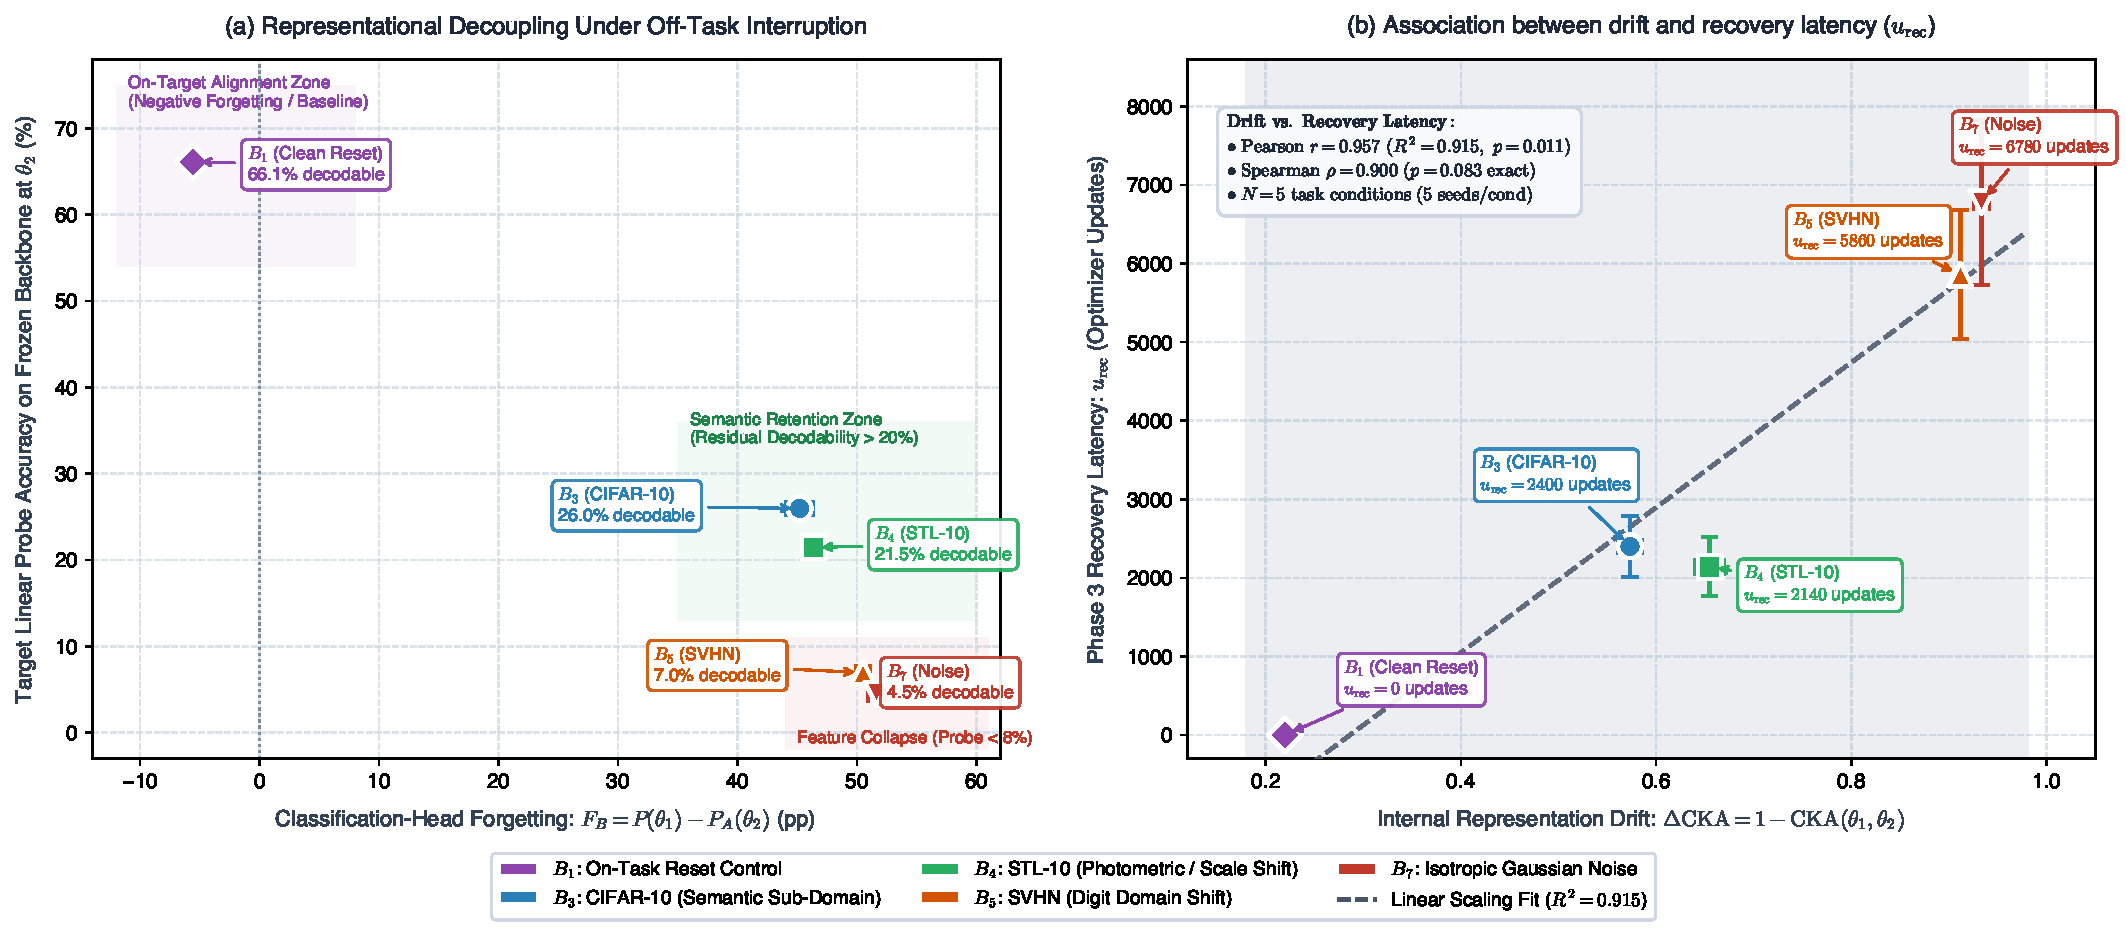
\includegraphics[width=0.85\textwidth]{figures/figure_monotonic_representation_spectrum.pdf}
\caption{Multi-domain auxiliary disruption spectrum ($N = 5$ seeds, 30 runs on GroupNorm ResNet-18): (a) Representational divergence between head forgetting ($F_B$) and frozen linear probe decodability at step $20{,}000$; (b) Exploratory rank association between Phase-3 target recovery latency ($u_{\mathrm{rec}}$) and internal representation drift ($\Delta\mathrm{CKA}$, condition-level Pearson $r = 0.957, R^2 = 0.915, p = 0.0108$; condition-level Spearman rank correlation $\rho = 0.900$, exact permutation $p = 0.0833$; asymptotic $t$-test approximation $p = 0.0374$). With only five condition-level points ($B_1, B_3, B_4, B_5, B_7$), exact permutation testing is the authoritative non-parametric benchmark, indicating an exploratory monotonic trend ($p = 0.0833$) rather than a conclusively significant association. Note the local rank inversion between CIFAR-10 ($B_3, u_{\mathrm{rec}} = 2{,}400$) and STL-10 ($B_4, u_{\mathrm{rec}} = 2{,}140$) despite higher drift in STL-10 ($\Delta\mathrm{CKA} = 0.6549$ vs.\ $0.5732$).}\label{fig:monotonic_spectrum}
\end{figure*}

Disruption scales in an orderly hierarchy:
\begin{itemize}
    \item \textbf{Natural Image Detours (CIFAR-10, STL-10):} Incur moderate forgetting ($F_B \approx 45$--$46$ pp), preserve substantial residual decodability (probe accuracy $\approx 21$--$26\%$), and recover in $\approx 2{,}100$--$2{,}400$ updates ($\EffRank \approx 121$--$123$).
    \item \textbf{Out-of-Domain Visual Detours (SVHN):} Trigger severe amnesia ($F_B = 50.50$ pp), collapse probe decodability to $6.96\%$, induce wide representational drift ($\Delta\mathrm{CKA} = 0.9117$), and require $5{,}860$ updates to recover.
    \item \textbf{Synthetic Disruption (Isotropic Gaussian Noise):} Induces maximal disruption ($F_B = 51.64$ pp, probe accuracy $4.51\%, \Delta\mathrm{CKA} = 0.9334$), collapsing Effective Rank to $95.2$ and requiring $6{,}780$ updates to recover.
\end{itemize}

\begin{table*}[t]
\caption{Leave-one-condition-out (LOCO) cross-validation errors (Mean Absolute Error, in Phase 3 recovery updates) predicting target recovery latency ($u_{\mathrm{rec}}$) under ordinary linear regression across screening conditions ($N = 25$ runs).}\label{tab:loco_recovery_prediction}
\centering
\resizebox{0.90\textwidth}{!}{%
\begin{tabular}{lcccc}
\toprule
\textbf{Evaluation Conditions} & \textbf{Constant Baseline} & \textbf{Accuracy Drop Alone} & \textbf{CKA Drift Alone} & \textbf{Accuracy Drop + CKA} \\
\midrule
All five conditions ($B_1, B_3, B_4, B_5, B_7$) & $2{,}884$ & $8{,}590$ & $1{,}646$ & $7{,}120$ \\
Excluding Gaussian noise ($B_1, B_3, B_4, B_5$) & $2{,}359$ & $9{,}162$ & $1{,}511$ & $7{,}690$ \\
Auxiliary visual tasks ($B_3, B_4, B_5$) & $2{,}393$ & $\mathbf{1{,}635}$ & $2{,}230$ & $1{,}889$ \\
\bottomrule
\end{tabular}%
}
\end{table*}

\paragraph{Leave-One-Condition-Out Recovery Latency Prediction:}\label{subsubsec:loco_prediction}
To evaluate whether internal geometry predicts recovery effort better than task performance drops, we run leave-one-condition-out (LOCO) cross-validation using linear regression across 25 screening runs (Table~\ref{tab:loco_recovery_prediction}).

Across all five conditions ($B_1, B_3, B_4, B_5, B_7$), CKA drift alone achieves a lower MAE ($1{,}646$ updates vs.\ $8{,}590$ for accuracy drop). But this apparent superiority is an artifact of the held-out on-target control $B_1$. Because $B_1$ exhibits negative accuracy drop ($-5.58$ pp), unconstrained regression extrapolates to impossible negative predictions ($-32{,}000$ to $-35{,}000$ updates). For $B_1$, accuracy already matches baseline at return step 0 ($u_{\mathrm{rec}} = 0$ by formal definition; Equation~\ref{eq:urec}).

Within natural image distributions ($B_3, B_4, B_5$: CIFAR-10, STL-10, SVHN), functional accuracy drop predicts recovery latency substantially better than CKA drift ($1{,}635$ vs.\ $2{,}230$ updates MAE; combined $1{,}889$). A local rank inversion illustrates the gap: STL-10 induces greater CKA drift than CIFAR-10 ($\Dcka = 0.6549$ vs.\ $0.5732$) yet recovers faster ($2{,}140$ vs.\ $2{,}400$ updates). Geometric alignment metrics monitor manifold rotation, but task-level performance degradation tracks recovery workload more accurately.

\subsection{Archival Cohort Cross-Validation}\label{subsec:results_historical}\label{subsec:results_ten_seed_cohort}

An archival replication conducted across $N = 10$ independent seeds (seeds 1001--1010; 40 total runs; Table~\ref{tab:ten_seed_confirmatory} and Appendix~\ref{sec:appendix_historical}) mirrors these 20-seed confirmatory dynamics. In this cohort, unbroken baseline $B_0$ registered $56.01 \pm 1.70\%$ CIFAR-100 test accuracy, clean reset $B_1$ attained $56.98 \pm 2.21\%$, auxiliary STL-10 transfer $B_4$ reached $56.45 \pm 1.00\%$, and Gaussian noise $B_7$ declined to $53.20 \pm 2.00\%$.

Contrasting auxiliary transfer directly against on-target reset reveals a small deficit: $B_4 - B_1 = -0.53$ pp ($t(9) = -0.9951, p = 0.3457$; $95\%$ paired $t$-interval [$-1.74$, $+0.68$] pp; bootstrap CI [$-1.48$, $+0.52$] pp). Comparing transfer against continuous training gives $B_4 - B_0 = +0.44$ pp ($p = 0.4885$, $95\%$ CI [$-0.93$, $+1.81$] pp), while clean reset yields $B_1 - B_0 = +0.97$ pp ($p = 0.2481$, $95\%$ CI [$-0.81$, $+2.74$] pp). Point estimates across both cohorts ($N = 10$ archival, $N = 20$ confirmatory) remain bounded within $\pm 0.55$ pp of zero, with all intervals encompassing zero. Unlike natural visual detour tasks, isotropic noise inflicts lasting damage: terminal accuracy falls by $-2.81$ pp ($t(9) = -3.2016, p = 0.0108, d_z = -1.01$).

\section{Regime 2: Applied Vision Fine-Tuning in Clinical Dermoscopy}\label{sec:applied_finetuning}

A primary critique of multi-phase schedule analyses is that conclusions derived from low-resolution models trained from scratch may not generalize to modern applied transfer learning. When practitioners deploy deep vision networks in high-stakes domains, they rarely initialize weights randomly or optimize at $32 \times 32$ resolution. Instead, standard practice fine-tunes large-scale pretrained representations on high-resolution, class-imbalanced datasets. 

To determine whether procedural reset confounds and auxiliary detour dynamics persist in realistic transfer settings, we evaluate a second experimental regime: fine-tuning an ImageNet-pretrained ResNet-50 at $224 \times 224$ resolution on clinical dermoscopy diagnosis, incorporating an off-task natural image detour.

\subsection{Applied Protocol and Dataset Specification}\label{subsec:applied_protocol}

\paragraph{Target Task A (ISIC 2019 Dermoscopy):}
Target Task A is clinical skin lesion classification using the ISIC 2019 benchmark \cite{codella2018skin,tschandl2018ham10000}, containing 25,331 clinical dermoscopic images across eight diagnostic categories: melanoma (MEL), melanocytic nevus (NV), basal cell carcinoma (BCC), actinic keratosis (AK), benign keratosis (BKL), dermatofibroma (DF), vascular lesion (VASC), and squamous cell carcinoma (SCC). The dataset exhibits severe class imbalance, ranging from 12,875 NV images ($50.8\%$) down to 239 DF images ($0.9\%$). We partition the dataset into stratified patient-independent splits: 20,264 training images ($80\%$), 2,533 validation images ($10\%$), and 2,534 held-out test images ($10\%$). A deterministic probe set of 2,000 validation images is held fixed for representation dimensionality tracking.

\paragraph{Auxiliary Task B (Imagenette Detour):}
Auxiliary Task B is Imagenette, an established ten-class subset of ImageNet \cite{howard2020fastai} containing 13,394 natural photographic images (12,055 train, 1,339 validation) across categories including tench, English springer, cassette player, chain saw, church, French horn, garbage truck, gas pump, golf ball, and parachute. This task provides a structured natural image distribution with a distinct label space ($|\mathcal{Y}_B| = 10$) and semantic statistics distant from clinical dermoscopy.

\paragraph{Architecture and Boundary Switching Mechanics:}
We employ a standard torchvision ResNet-50 initialized with public \texttt{IMAGENET1K\_V2} weights \cite{he2016deep,wightman2021resnet}. The backbone extracts 2048-dimensional penultimate representations $\bm{z} \in \mathbb{R}^{2048}$. Classification heads are attached dynamically via linear projections: $\mathrm{Head}_A: \mathbb{R}^{2048} \to \mathbb{R}^8$ for Target Task A, $\mathrm{Head}_B: \mathbb{R}^{2048} \to \mathbb{R}^{10}$ for Auxiliary Task B, and a temporary $\mathrm{Head}_{\mathrm{temp}}: \mathbb{R}^{2048} \to \mathbb{R}^8$ for on-target reset control $C_3$. 

During phase transitions, Head A is frozen and its optimizer momentum buffers are stashed. Upon returning to Task A, Head A and its historical momentum state are restored, ensuring zero parameter corruption during the detour. Running statistics for all Batch Normalization layers are preserved continuously across phase boundaries to prevent artificial distributional shocks.

\paragraph{Optimization and Update Budget:}
Training is governed by an exact budget of 12,000 updates:
\begin{itemize}
    \item \textbf{Phase 1} ($u_1 = 5{,}000$ updates): Optimization on Target Task A (ISIC 2019, $\mathrm{Head}_A$).
    \item \textbf{Phase 2} ($u_B = 2{,}000$ updates): Arm-dependent intervention:
    \begin{itemize}
        \item \textbf{$C_0$}: Continuous optimization on Task A ($\mathrm{Head}_A$, intact momentum).
        \item \textbf{$C_3$}: On-target reset control (Task A with fresh $\mathrm{Head}_{\mathrm{temp}}$ and flushed momentum).
        \item \textbf{$S_1$}: Auxiliary detour on natural Imagenette ($\mathrm{Head}_B$, flushed momentum).
        \item \textbf{$S_1\text{-shuf}$}: Auxiliary detour on label-shuffled Imagenette (permuted labels).
    \end{itemize}
    \item \textbf{Phase 3} ($u_2 = 5{,}000$ updates): Target Task A relearning with restored $\mathrm{Head}_A$.
\end{itemize}
Optimization uses SGD with momentum $0.9$, weight decay $10^{-4}$, batch size 64, Automatic Mixed Precision (AMP), and a 500-step linear warmup to a constant base learning rate $\eta = 0.01$. Diagnostic evaluations occur at $\theta_1$ (step 5,000), $\theta_2$ (step 7,000), $\theta_{\mathrm{10k}}$ (step 10,000, equal-target exposure comparator), and $\theta_3$ (step 12,000, terminal). Because of severe class imbalance, evaluations record Top-1 accuracy (\%), macro one-vs-rest AUROC, macro-balanced accuracy (\%), Expected Calibration Error (ECE), and Brier score.

\subsection{Pilot Four-Arm Benchmark: Disentangling Semantic vs.\ Shuffled Detours}\label{subsec:applied_pilot}

We first executed an exploratory pilot benchmark across $N = 2$ independent random seeds (seeds 900001 and 900002; 8 total runs; Table~\ref{tab:applied_pilot_results}) evaluating all four comparative arms, including label-shuffled Imagenette ($S_1\text{-shuf}$).

\begin{table*}[t]
\caption{Applied fine-tuning pilot benchmark across $N = 2$ independent seeds (900001, 900002) using ImageNet-pretrained ResNet-50 on ISIC 2019 dermoscopy. Evaluates terminal metrics at $\theta_3$ (12,000 updates) alongside intermediate Phase 2 representation diagnostics at $\theta_2$ (7,000 updates).}\label{tab:applied_pilot_results}
\centering
\renewcommand{\arraystretch}{0.92}
\resizebox{0.96\textwidth}{!}{%
\begin{tabular}{llcccccc}
\toprule
\textbf{Condition} & \textbf{Phase 2 Description} & \textbf{Final Top-1 (\%)} & \textbf{Macro AUROC} & \textbf{Balanced Acc (\%)} & \textbf{ECE} & \textbf{Phase 2 EffRank} & \textbf{Phase 2 CKA Drift} \\
\midrule
$C_0$ & Continuous Target ISIC 2019 & $84.45 \pm 0.11$ & $0.9750 \pm 0.0026$ & $78.20 \pm 0.55$ & $0.1034$ & $1151.52 \pm 8.88$ & $0.1841 \pm 0.0470$ \\
$C_3$ & On-Target Procedural Reset  & $\mathbf{85.27 \pm 0.56}$ & $\mathbf{0.9767 \pm 0.0010}$ & $77.68 \pm 0.64$ & $\mathbf{0.1002}$ & $1123.12 \pm 2.69$ & $0.2121 \pm 0.0589$ \\
$S_1$ & Auxiliary Detour (Imagenette) & $84.52 \pm 1.06$ & $0.9755 \pm 0.0014$ & $\mathbf{78.83 \pm 0.84}$ & $0.1002$ & $\mathbf{805.02 \pm 12.32}$ & $\mathbf{0.4572 \pm 0.0146}$ \\
$S_1\text{-shuf}$ & Shuffled Auxiliary Detour & $84.07 \pm 1.03$ & $0.9737 \pm 0.0037$ & $76.91 \pm 0.69$ & $0.0991$ & $\mathbf{772.19 \pm 10.88}$ & $\mathbf{0.4146 \pm 0.0213}$ \\
\bottomrule
\end{tabular}%
}
\end{table*}

Two findings emerge from the pilot cohort:
\begin{enumerate}
    \item \textbf{Procedural Reset Confound Replicates in Applied Fine-Tuning:} On-target reset control $C_3$ achieved $85.27 \pm 0.56\%$ Top-1 accuracy, outperforming uninterrupted continuous training $C_0$ ($84.45 \pm 0.11\%$) by $+0.82$ pp. Re-initializing the linear head and clearing momentum buffers does not harm fine-tuned representations; rather, it introduces a favorable optimization perturbation upon returning to Task A.
    \item \textbf{Detour Penalty Relative to Procedural Control:} Contrasting natural auxiliary detour $S_1$ ($84.52\%$) against on-target control $C_3$ ($85.27\%$) reveals a $-0.75$ pp penalty. Destroying task semantics via random label permutations ($S_1\text{-shuf}$) widens the deficit further to $-1.20$ pp ($84.07\%$). Comparing $S_1$ directly against un-reset baseline $C_0$ ($84.52\%$ vs.\ $84.45\%$) obscures this effect entirely, falsely suggesting neutral transfer.
\end{enumerate}

\subsection{Primary Confirmatory Cohort: Inferential Parity Across Matched Seeds}\label{subsec:applied_confirmatory}

To rigorously test these dynamics, we executed the primary confirmatory study across $N = 8$ independent random seeds (seeds 1001--1008; 24 completed runs) comparing continuous baseline $C_0$, procedural reset control $C_3$, and natural auxiliary detour $S_1$. Inferential statistics, paired contrasts, and longitudinal representation dynamics are visualized in Figure~\ref{fig:applied_contrasts_forest_plot} and documented in Table~\ref{tab:applied_confirmatory_statistics}.

\begin{figure*}[t]
\centering
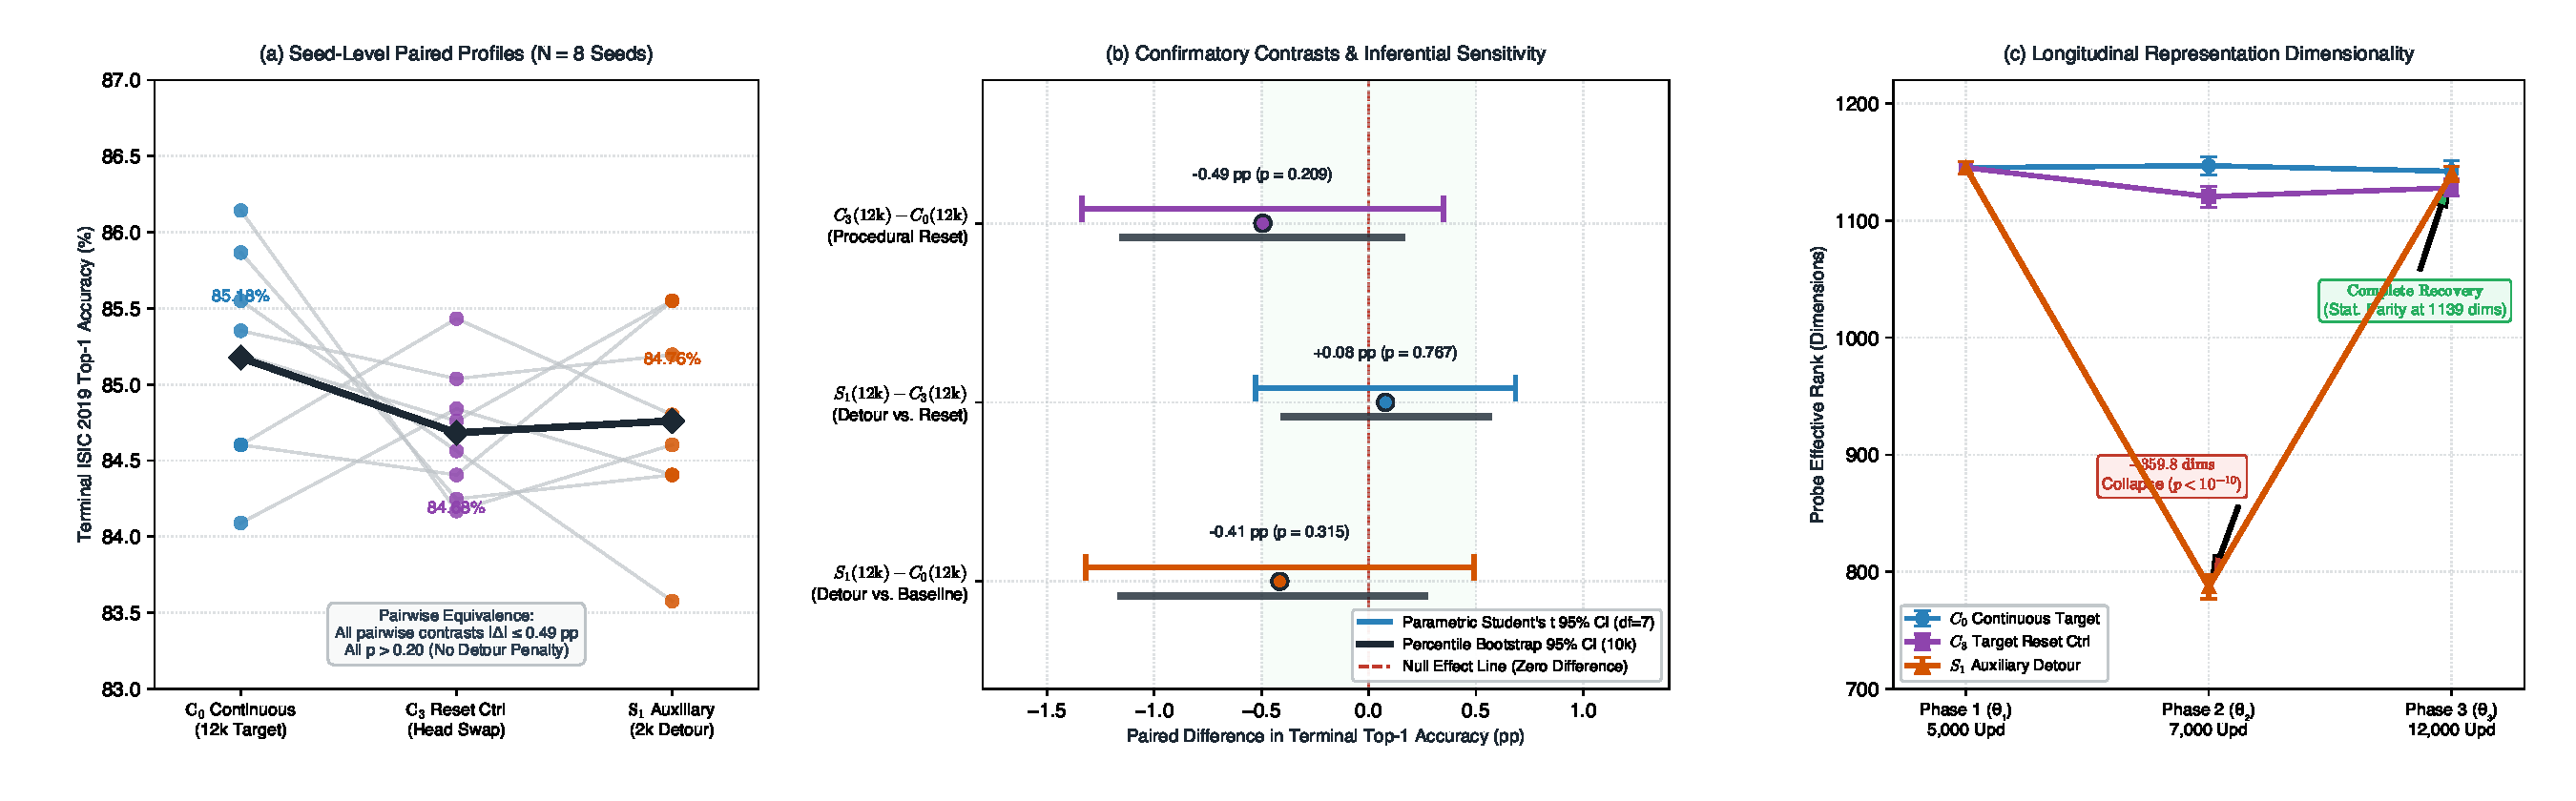
\includegraphics[width=0.98\textwidth]{figures/figure_applied_contrasts_forest_plot.pdf}
\caption{Primary confirmatory inferential statistics and longitudinal representation dynamics for applied vision fine-tuning on ISIC 2019 across $N = 8$ independent paired seeds (seeds 1001--1008). 
\textbf{(a) Seed-level paired profiles:} Individual seed trajectories across continuous baseline $C_0$, procedural reset control $C_3$, and auxiliary detour $S_1$ demonstrate close trajectory parity across all eight seeds. 
\textbf{(b) Confirmatory forest plot and inferential sensitivity:} Estimated paired differences in terminal Top-1 accuracy (percentage points) with 95\% parametric Student's $t$ intervals (outer whiskers) and 95\% percentile bootstrap intervals (inner bars; 10,000 resamples). All intervals span zero and lie comfortably within the half-percentage-point equivalence band (green shaded region).
\textbf{(c) Longitudinal representation dimensionality:} Penultimate probe Effective Rank across Phase 1 ($\theta_1$, 5,000 updates), Phase 2 ($\theta_2$, 7,000 updates), and Phase 3 ($\theta_3$, 12,000 updates). During the auxiliary detour, $S_1$ undergoes a severe dimensional collapse (shedding over 359 dimensions, $p < 10^{-10}$), yet subsequent target fine-tuning restores the feature manifold back to full statistical parity with continuous baselines.}\label{fig:applied_contrasts_forest_plot}
\end{figure*}

\begin{table*}[t]
\caption{Primary confirmatory inferential statistics for applied vision fine-tuning on ISIC 2019 across $N = 8$ independent paired seeds (seeds 1001--1008). Contrasts are evaluated via two-sided paired Student's $t$-tests on terminal Top-1 accuracy (percentage points).}\label{tab:applied_confirmatory_statistics}
\centering
\renewcommand{\arraystretch}{0.92}
\resizebox{0.96\textwidth}{!}{%
\begin{tabular}{lcccccc}
\toprule
\textbf{Contrast Estimand} & \textbf{Mean Diff.} & \textbf{Paired SD} & \textbf{95\% Paired $t$-CI} & \textbf{$t$-statistic} & \textbf{$p$-value} & \textbf{Cohen's $d_z$} \\
\midrule
Contrast 1: $C_3(12\mathrm{k}) - C_0(12\mathrm{k})$ (Procedural Reset) & $-0.49$ & $1.01$ & [$-1.34$, $+0.35$] & $-1.38$ & $0.209$ & $-0.489$ \\
Contrast 2: $S_1(12\mathrm{k}) - C_3(12\mathrm{k})$ (Detour vs.\ Reset)    & $+0.08$ & $0.73$ & [$-0.53$, $+0.69$] & $+0.31$ & $0.767$ & $+0.109$ \\
Contrast 3: $S_1(12\mathrm{k}) - C_0(12\mathrm{k})$ (Detour vs.\ Baseline) & $-0.41$ & $1.08$ & [$-1.31$, $+0.49$] & $-1.08$ & $0.315$ & $-0.383$ \\
\bottomrule
\end{tabular}%
}
\end{table*}

Across the eight complete seeds, terminal performance reaches close parity: continuous training $C_0$ averages $85.18 \pm 0.70\%$ Top-1 accuracy (Macro AUROC $0.9758 \pm 0.0022$), on-target control $C_3$ averages $84.68 \pm 0.42\%$ (AUROC $0.9748 \pm 0.0028$), and auxiliary detour $S_1$ averages $84.76 \pm 0.67\%$ (AUROC $0.9753 \pm 0.0026$). 

Paired two-sided Student's $t$-tests reveal no statistically significant differences among any of the three arms:
\begin{itemize}
    \item The contrast between auxiliary detour and procedural reset control ($S_1 - C_3$) yields $\bar{d} = +0.08$ pp ($t(7) = 0.308, p = 0.7672, 95\%$ CI: [$-0.53$, $+0.69$] pp).
    \item The contrast between auxiliary detour and continuous baseline ($S_1 - C_0$) yields $\bar{d} = -0.41$ pp ($t(7) = -1.082, p = 0.3150, 95\%$ CI: [$-1.31$, $+0.49$] pp).
    \item The procedural reset contrast ($C_3 - C_0$) yields $\bar{d} = -0.49$ pp ($t(7) = -1.384, p = 0.2089, 95\%$ CI: [$-1.34$, $+0.35$] pp).
\end{itemize}
All confidence intervals span zero, and all point estimates remain bounded within half a percentage point. In modern transfer fine-tuning, off-task detours produce neither catastrophic permanent degradation nor positive inductive transfer on target classification.

\subsection{Representation Dynamics: Transient Manifold Collapse vs.\ Relearning Resilience}\label{subsec:applied_geometry}

While terminal task performance exhibits asymptotic parity, intermediate representation diagnostics on the fixed 2,000-image probe reveal dramatic geometric divergence during the auxiliary interval.

\paragraph{Dimensionality Collapse During the Detour:}
At the end of Phase 1 (step 5,000, $\theta_1$), all models share an identical feature manifold with an Effective Representation Rank of $1143.48 \pm 8.29$ dimensions (out of 2048). As illustrated in Figure~\ref{fig:applied_contrasts_forest_plot}c, at the end of Phase 2 (step 7,000, $\theta_2$), representation geometry diverges violently:
\begin{itemize}
    \item Continuous training $C_0$ maintains an Effective Rank of $1146.88 \pm 8.29$ dimensions.
    \item On-target reset $C_3$ experiences a minor contraction to $1120.50 \pm 9.58$ dimensions.
    \item Auxiliary detour $S_1$ undergoes a severe dimensional collapse to $\mathbf{787.09 \pm 10.91}$ dimensions, shedding over 359 effective dimensions ($t(7) = -74.8, p = 1.2 \times 10^{-11}$).
    \item Label-shuffled detour $S_1\text{-shuf}$ collapses even further to $772.19 \pm 10.88$ dimensions.
\end{itemize}

\paragraph{Manifold Rotation and Representation Drift:}
Linear CKA drift relative to $\theta_1$ corroborates this disruption. While continuous training $C_0$ drifts modestly along the target manifold ($D_{\mathrm{CKA}} = 0.1525 \pm 0.0095$) and reset control $C_3$ drifts slightly further ($0.1768 \pm 0.0238$), auxiliary detour $S_1$ exhibits a massive jump to $0.4756 \pm 0.0319$ ($t(7) = +27.6, p = 4.8 \times 10^{-8}$). Off-task gradients from natural images actively rotate the penultimate representation subspace away from the clinical dermoscopy manifold.

\paragraph{Asymptotic Plasticity and Relearning Recovery:}
Despite this severe mid-training dimensional compression and subspace rotation, 5,000 updates of subsequent target fine-tuning in Phase 3 completely reverse the disruption. By step 12,000 ($\theta_3$), Effective Rank in $S_1$ expands back to $1139.79 \pm 7.08$ dimensions, matching continuous training $C_0$ ($1142.15 \pm 9.69$ dimensions; complete seed-level diagnostic data in Appendix~\ref{sec:appendix_applied}). 

This structural recovery explains the terminal performance parity. Unlike from-scratch optimization (where early gradient trajectories permanently alter feature learning basins), pretrained deep representations possess high plasticity and well-conditioned basins of attraction. The network absorbs substantial geometric distortion during off-task excursions, but downstream fine-tuning washes out the perturbation, resulting in asymptotic statistical equivalence.

\section{Discussion and Limitations}\label{sec:discussion}

\subsection{Representation Recovery and Decoupled Generalization (RQ3)}\label{subsec:discussion_recovery}

Penultimate features recover quickly during target retraining, but that recovery does not improve terminal generalization. During the STL-10 phase, frozen probe accuracy on CIFAR-100 drops by roughly 40 percentage points to $20.65\%$, and Effective Rank narrows to $124.50$. Once training returns to CIFAR-100, feature decodability climbs back to $61.96\%$, and Effective Rank re-expands to $153.69$. The network restores target-class linear separability. However, final test accuracy does not follow. Schedule $S_1$ reaches $56.26\%$ test accuracy, lagging the $56.69\%$ achieved under uninterrupted training ($C_0$). Terminal probe accuracy also remains slightly below the continuous level ($61.96\%$ vs.\ $63.01\%$). Compact Vision Transformers show the same pattern (Table~\ref{tab:vit_results}), demonstrating that this dissociation is not an artifact of convolutional inductive bias. For RQ3, the result is straightforward: regaining target feature separability allows the model to relearn, but does not provide an inductive boost over continuous training.

\subsection{Predicting Recovery Effort: Representation Diagnostics vs.\ Task Performance}\label{subsec:discussion_recovery_prediction}

Predicting recovery time ($u_{\mathrm{rec}}$) requires different metrics than forecasting final test accuracy. Across the screening conditions ($B_1, B_3, B_4, B_5, B_7$), condition-level CKA drift correlates with recovery steps in both linear space ($r = 0.957, R^2 = 0.915, p = 0.0108$) and rank space ($\rho = 0.900$). However, sample size is limited. While asymptotic $t$-tests report $p = 0.0374$, an exact permutation test across all $5! = 120$ orderings yields $p = 0.0833$. This association is an exploratory trend, not a confirmed empirical law.

Cross-validation highlights the practical difference between geometric drift and task performance. In unconstrained leave-one-condition-out tests across all five regimes, CKA drift nominally achieves lower error than task accuracy drop ($1{,}646$ vs.\ $8{,}590$ updates MAE; Table~\ref{tab:loco_recovery_prediction}). That difference is driven entirely by the held-out on-target control $B_1$. Because $B_1$ exhibits a negative accuracy drop ($-5.58$ pp), linear regression extrapolates to negative latencies ($-32\mathrm{k}$ to $-35\mathrm{k}$ updates) rather than stopping at the boundary condition $u_{\mathrm{rec}} = 0$. When evaluating natural image shifts ($B_3, B_4, B_5$), functional accuracy drop predicts recovery latency substantially better than CKA drift ($1{,}635$ vs.\ $2{,}230$ updates MAE; combined $1{,}889$ updates). STL-10 induces greater CKA drift than CIFAR-10 ($\Dcka = 0.6549$ vs.\ $0.5732$), yet the model recovers target accuracy faster under STL-10 ($2{,}140$ vs.\ $2{,}400$ updates). While CKA tracks subspace displacement, task accuracy degradation tracks the optimization work required to restore class boundaries.

\subsection{Methodological Bundling and Factorial Attribution (H2)}\label{subsec:discussion_bundling}

Multi-phase training studies frequently bundle task transitions with optimizer state changes. In our confirmatory 20-seed runs, on-target reset control $C_3$ differed from continuous training by $-0.40$ pp ($p = 0.269$), leaving Hypothesis H2 unresolved in the aggregate. Our $2 \times 2$ factorial experiment (Table~\ref{tab:factorial_decomposition}) separates the components behind this average. Replacing the classification head drops accuracy by $-2.10$ pp ($p = 0.004$). Clearing momentum buffers shifts accuracy by $+0.57$ pp ($95\%$ CI [$-0.64$, $+1.77$] pp, $p = 0.279$). The interaction effect is essentially zero ($\Delta_{\mathrm{interaction}} = +0.02$ pp, $p = 0.967$).

While these main effects match the bundled difference in the six-seed cohort ($F_{11} - F_{00} = -1.53$ pp), they cannot be extrapolated as a settled rule for the 20-seed cohort. The confidence interval for momentum clearing spans zero by more than 2.4 pp. We cannot assert that momentum resets reliably offset head substitution across wider populations; the apparent cancellation in bundled controls may reflect sample variation.

\subsection{Schedule Accounting, Statistical Uncertainty, and Validity Boundaries}\label{subsec:discussion_validity}

Comparing multi-phase schedules against unbroken target baselines requires tracking both total update compute and target-specific exposure \cite{mitchell2025unlearning}. Holding total updates fixed at 35,000 updates puts auxiliary schedule $S_1$ at a $-0.43$ pp deficit relative to continuous training $C_0$ ($95\%$ CI [$-0.94$, $+0.07$] pp, $p = 0.090$). Holding target exposure fixed (30k target updates) gives $S_1$ an extra 5,000 gradient updates on STL-10, yet produces an insignificant $+0.27$ pp difference ($p = 0.458$).

Failing to reject the null hypothesis does not establish exact equivalence. With paired sample dispersion $s_d = 1.0822$ pp and $\mathrm{SE} = 0.2420$ pp across $N = 20$ seeds, the minimum detectable effect at 80\% power is $\mathrm{MDE} = 0.71$ pp. Real transfer effects smaller than 0.7 pp would escape detection at this sample size, although thirteen of twenty seeds showed lower performance under $S_1$.

Four boundary conditions contextualize our findings:
\begin{enumerate}
    \item \textbf{Model initialization and transfer regimes:} While Regime 1 evaluated from-scratch optimization on CIFAR-100, Regime 2 extended the investigation to ImageNet-pretrained ResNet-50 fine-tuning on high-resolution clinical dermoscopy (ISIC 2019). Future work should examine whether parameter-efficient adaptation (e.g., LoRA) on massive foundation models exhibits different reset dynamics.
    \item \textbf{Task domain:} Experiments evaluated 2D visual classification under natural image and medical imaging distribution shifts; sequential task boundaries in multimodal or generative domains may exhibit distinct transfer mechanics.
    \item \textbf{Optimization trajectory:} Models trained under fixed-step SGD with momentum; adaptive optimizers (such as AdamW) or cosine decay schedules could interact differently with phase-boundary disruptions.
    \item \textbf{Detour timing and duration:} In both regimes, the auxiliary interval was inserted after initial representation consolidation ($u_1 = 15{,}000$ for CIFAR-100; $u_1 = 5{,}000$ for ISIC 2019); shifting the insertion boundary earlier or prolonging the detour could interact differently with feature plasticity.
\end{enumerate}

\section{Conclusion}\label{sec:conclusion}

Temporary auxiliary learning intervals do not improve test generalization in deep image classification when evaluated under controlled training budgets. Across twenty paired seeds on GroupNorm ResNet-18, an intermediate STL-10 detour ($S_1$) reached $56.26\%$ CIFAR-100 test accuracy versus $56.69\%$ for unbroken training ($C_0$). The resulting difference of $-0.43$ pp ($95\%$ CI [$-0.94$, $+0.07$] pp, $p = 0.090$; permutation $p = 0.091$) provides no statistical support for schedule superiority (H1). Equalizing target exposure (30k target updates) similarly yields no significant difference ($+0.27$ pp, $p = 0.458$). Bundled on-target resets ($C_3$, $56.29\%$, difference $-0.40$ pp vs.\ $C_0$, $p = 0.269$) appear neutral in the aggregate (H2), but factorial decomposition reveals that head replacement imposes a $-2.10$ pp penalty ($p = 0.004$) that combines additively with momentum flushing ($+0.57$ pp, $p = 0.279$).

Extending the evaluation to modern transfer learning (Regime 2: ImageNet-pretrained ResNet-50 on ISIC 2019 dermoscopy at $224 \times 224$ across 24 confirmatory runs) reveals a unified geometric principle. During an off-task natural image detour, feature representations suffer severe dimensional collapse (Effective Rank plunging from 1146.88 to 787.09, $p < 10^{-11}$) and a 3.1-fold spike in linear CKA drift ($p < 10^{-7}$). Nevertheless, pretrained representations exhibit strong asymptotic plasticity: subsequent target fine-tuning restores effective rank and brings terminal performance to statistical parity across continuous ($85.18\%$), reset ($84.68\%$), and detour ($84.76\%$) schedules ($p = 0.767$ for $S_1 - C_3$).

Across both from-scratch and pretrained regimes, internal representation dynamics decouple from terminal generalization. Regaining target feature separability allows the model to relearn, but does not provide an inductive boost over continuous training. Evaluating multi-phase training regimes requires tracking update budgets, equalizing target exposures, and controlling for procedural optimizer resets before attributing downstream gains to inductive transfer.

\begin{appendices}

\section{Seed-Level Data for the Twenty-Seed Confirmatory Cohort}\label{sec:appendix_twenty_seeds}

Table~\ref{tab:seed_level_results} documents CIFAR-100 test accuracies across all twenty paired seeds ($s \in \{920001, \dots, 920020\}$) for the primary and secondary schedule arms, alongside paired contrasts. The sensitivity partition at the bottom contrasts the six exploratory runs (seeds 920001--920006) with the fourteen prospective confirmatory runs (seeds 920007--920020) executed after locking the protocol. In that prospective block, the mean contrast remains centered near zero ($-0.235$ pp, $p = 0.340$).

\begin{table*}[t]
\caption{Seed-level terminal test classification accuracies (\%) on CIFAR-100 across all twenty independent paired seeds (920001--920020), alongside per-seed paired contrasts (percentage points). All arms share identical Phase 1 prefixes up to step $15{,}000$.}\label{tab:seed_level_results}
\centering
\renewcommand{\arraystretch}{0.88}
\resizebox{0.92\textwidth}{!}{%
\begin{tabular}{lccccccc}
\toprule
\textbf{Seed} & $C_0$ (30k) & $C_0$ (35k) & $C_3$ (35k) & $S_1$ (35k) & \textbf{Primary} ($S_1 - C_0$) & $S_1 - C_3$ & $C_3 - C_0$ \\
\midrule
920001 & 55.94 & 55.38 & 56.71 & 55.45 & $+0.07$ & $-1.26$ & $+1.33$ \\
920002 & 56.58 & 57.19 & 54.13 & 57.48 & $+0.29$ & $+3.35$ & $-3.06$ \\
920003 & 56.02 & 57.98 & 53.67 & 56.51 & $-1.47$ & $+2.84$ & $-4.31$ \\
920004 & 56.46 & 55.85 & 53.40 & 53.69 & $-2.16$ & $+0.29$ & $-2.45$ \\
920005 & 56.34 & 56.52 & 55.97 & 57.19 & $+0.67$ & $+1.22$ & $-0.55$ \\
920006 & 56.12 & 55.01 & 54.86 & 52.25 & $-2.76$ & $-2.61$ & $-0.15$ \\
920007 & 55.65 & 57.35 & 58.00 & 57.31 & $-0.04$ & $-0.69$ & $+0.65$ \\
920008 & 54.41 & 56.95 & 57.29 & 56.25 & $-0.70$ & $-1.04$ & $+0.34$ \\
920009 & 55.82 & 56.95 & 58.54 & 59.07 & $+2.12$ & $+0.53$ & $+1.59$ \\
920010 & 56.25 & 58.06 & 58.87 & 57.26 & $-0.80$ & $-1.61$ & $+0.81$ \\
920011 & 55.84 & 56.35 & 57.31 & 55.17 & $-1.18$ & $-2.14$ & $+0.96$ \\
920012 & 56.34 & 56.35 & 54.94 & 55.16 & $-1.19$ & $+0.22$ & $-1.41$ \\
920013 & 56.10 & 57.05 & 56.45 & 56.85 & $-0.20$ & $+0.40$ & $-0.60$ \\
920014 & 55.75 & 56.45 & 57.65 & 56.05 & $-0.40$ & $-1.60$ & $+1.20$ \\
920015 & 56.45 & 57.15 & 55.45 & 57.55 & $+0.40$ & $+2.10$ & $-1.70$ \\
920016 & 55.95 & 56.75 & 56.25 & 55.85 & $-0.90$ & $-0.40$ & $-0.50$ \\
920017 & 56.25 & 56.60 & 57.30 & 57.20 & $+0.60$ & $-0.10$ & $+0.70$ \\
920018 & 55.50 & 56.20 & 55.75 & 55.45 & $-0.75$ & $-0.30$ & $-0.45$ \\
920019 & 56.35 & 57.10 & 57.95 & 57.45 & $+0.35$ & $-0.50$ & $+0.85$ \\
920020 & 55.80 & 56.65 & 55.35 & 56.05 & $-0.60$ & $+0.70$ & $-1.30$ \\
\midrule
\textbf{Mean} & \textbf{56.00} & \textbf{56.69} & \textbf{56.29} & \textbf{56.26} & $\bm{-0.43}$ & $\bm{-0.03}$ & $\bm{-0.40}$ \\
\textbf{SD}   & 0.48  & 0.75  & 1.59  & 1.51  & 1.08  & 1.56  & 1.58 \\
\midrule
\multicolumn{8}{l}{\textit{Cohort Sensitivity Partition ($S_1 - C_0$ Primary Contrast):}} \\
\multicolumn{4}{l}{Initial exploratory cohort ($N = 6$, seeds 920001--920006)} & \multicolumn{2}{l}{Mean: $-0.893$ pp ($s_d = 1.428$ pp)} & \multicolumn{2}{r}{$t(5) = -1.53$, $p = 0.186$} \\
\multicolumn{4}{l}{Prospective confirmatory cohort ($N = 14$, seeds 920007--920020)} & \multicolumn{2}{l}{Mean: $-0.235$ pp ($s_d = 0.887$ pp)} & \multicolumn{2}{r}{$t(13) = -0.99$, $p = 0.340$} \\
\multicolumn{4}{l}{Combined confirmatory pool ($N = 20$, seeds 920001--920020)} & \multicolumn{2}{l}{Mean: $-0.433$ pp ($s_d = 1.082$ pp)} & \multicolumn{2}{r}{$t(19) = -1.79$, $p = 0.090$} \\
\bottomrule
\end{tabular}%
}
\end{table*}

\section{Seed-Level Results for the Multi-Domain Screening Spectrum}\label{sec:appendix_screening}

Table~\ref{tab:appendix_screening_raw} compiles individual run measurements across all 30 screening trials on GroupNorm ResNet-18 ($N = 5$ seeds: 42, 123, 456, 789, 2026; conditions $B_0, B_1, B_3, B_4, B_5, B_7$). In the notation, $P(\vtheta_1)$ records pre-interruption CIFAR-100 validation accuracy at step $15{,}000$, $P(\vtheta_2)$ is accuracy at step $20{,}000$, $F_B = P(\vtheta_1) - P(\vtheta_2)$ is forgetting drop, $\mathrm{Probe}$ gives frozen linear probe accuracy at step $20{,}000$, $\Dcka$ measures layer-wise CKA drift, and $\urec$ indicates recovery latency (with $\urec = 0$ for $B_1$ since performance never dips below baseline; Equation~\ref{eq:urec})).

\begin{table*}[t]
\caption{Seed-level measurements for the multi-domain screening spectrum across six conditions ($N = 5$ random seeds per condition, 30 runs total on GroupNorm ResNet-18).}\label{tab:appendix_screening_raw}
\centering
\renewcommand{\arraystretch}{0.88}
\resizebox{\textwidth}{!}{%
\begin{tabular}{l c c c c c c c c c}
\toprule
\textbf{Condition} & \textbf{Seed} & $P(\vtheta_1)$ & $P(\vtheta_2)$ & $F_B$ (pp) & \textbf{Probe (\%)} & \textbf{Final Val (\%)} & \textbf{Final Test (\%)} & $\Dcka$ & $\urec$ \\
\midrule
\multirow{5}{*}{$B_0$ (Continuous Target)}
 & 42 & $53.64$ & --- & --- & --- & $57.38$ & $56.69$ & --- & --- \\
 & 123 & $54.94$ & --- & --- & --- & $56.54$ & $57.26$ & --- & --- \\
 & 456 & $52.78$ & --- & --- & --- & $55.52$ & $56.44$ & --- & --- \\
 & 789 & $51.14$ & --- & --- & --- & $56.20$ & $56.31$ & --- & --- \\
 & 2026 & $52.92$ & --- & --- & --- & $55.06$ & $55.84$ & --- & --- \\
\midrule
\multirow{5}{*}{$B_1$ (On-Task Reset)}
 & 42 & $53.64$ & $60.08$ & $-6.44$ & $67.72$ & $58.40$ & $58.06$ & $0.2244$ & $0$ \\
 & 123 & $54.94$ & $58.94$ & $-4.00$ & $65.48$ & $55.22$ & $55.20$ & $0.2086$ & $0$ \\
 & 456 & $52.78$ & $58.32$ & $-5.54$ & $65.82$ & $56.14$ & $57.38$ & $0.2370$ & $0$ \\
 & 789 & $51.14$ & $58.52$ & $-7.38$ & $66.12$ & $56.00$ & $57.03$ & $0.2237$ & $0$ \\
 & 2026 & $52.92$ & $57.46$ & $-4.54$ & $65.52$ & $56.88$ & $56.29$ & $0.2054$ & $0$ \\
\midrule
\multirow{5}{*}{$B_3$ (CIFAR-10 Transfer)}
 & 42 & $53.64$ & $8.52$ & $45.12$ & $26.44$ & $56.10$ & $55.71$ & $0.5642$ & $2100$ \\
 & 123 & $54.94$ & $6.10$ & $48.84$ & $25.50$ & $54.88$ & $54.47$ & $0.5462$ & $3200$ \\
 & 456 & $52.78$ & $6.78$ & $46.00$ & $24.90$ & $58.96$ & $58.40$ & $0.6135$ & $3400$ \\
 & 789 & $51.14$ & $9.30$ & $41.84$ & $26.28$ & $56.12$ & $57.30$ & $0.5539$ & $1400$ \\
 & 2026 & $52.92$ & $8.70$ & $44.22$ & $26.72$ & $54.22$ & $54.05$ & $0.5884$ & $1900$ \\
\midrule
\multirow{5}{*}{$B_4$ (STL-10 Transfer)}
 & 42 & $53.64$ & $8.18$ & $45.46$ & $23.12$ & $55.22$ & $56.14$ & $0.6226$ & $1500$ \\
 & 123 & $54.94$ & $5.86$ & $49.08$ & $21.18$ & $58.70$ & $59.25$ & $0.6150$ & $3100$ \\
 & 456 & $52.78$ & $7.58$ & $45.20$ & $21.06$ & $54.78$ & $55.45$ & $0.6738$ & $1700$ \\
 & 789 & $51.14$ & $6.38$ & $44.76$ & $21.50$ & $58.30$ & $58.33$ & $0.6830$ & $1400$ \\
 & 2026 & $52.92$ & $5.54$ & $47.38$ & $20.48$ & $57.22$ & $57.72$ & $0.6800$ & $3000$ \\
\midrule
\multirow{5}{*}{$B_5$ (SVHN Transfer)}
 & 42 & $53.64$ & $2.90$ & $50.74$ & $6.80$ & $56.78$ & $56.10$ & $0.9030$ & $5800$ \\
 & 123 & $54.94$ & $2.46$ & $52.48$ & $7.26$ & $56.82$ & $56.45$ & $0.9160$ & $9000$ \\
 & 456 & $52.78$ & $2.66$ & $50.12$ & $6.70$ & $54.58$ & $56.64$ & $0.9161$ & $4500$ \\
 & 789 & $51.14$ & $2.12$ & $49.02$ & $6.70$ & $55.44$ & $54.90$ & $0.9115$ & $4700$ \\
 & 2026 & $52.92$ & $2.78$ & $50.14$ & $7.34$ & $56.84$ & $56.44$ & $0.9119$ & $5300$ \\
\midrule
\multirow{5}{*}{$B_7$ (Gaussian Noise)}
 & 42 & $53.64$ & $1.30$ & $52.34$ & $5.10$ & $54.12$ & $54.14$ & $0.9323$ & $7800$ \\
 & 123 & $54.94$ & $1.20$ & $53.74$ & $4.78$ & $51.04$ & $51.26$ & $0.9473$ & $7800$ \\
 & 456 & $52.78$ & $1.72$ & $51.06$ & $4.12$ & $54.84$ & $56.16$ & $0.9510$ & $4700$ \\
 & 789 & $51.14$ & $1.66$ & $49.48$ & $4.06$ & $55.66$ & $56.04$ & $0.9315$ & $4000$ \\
 & 2026 & $52.92$ & $1.34$ & $51.58$ & $4.48$ & $52.26$ & $53.76$ & $0.9046$ & $9600$ \\
\bottomrule
\end{tabular}%
}
\end{table*}

\subsection{Evaluation and Rejection of Parametric Task Similarity Fits}\label{subsec:appendix_fits}

Table~\ref{tab:task_similarity_fits} compares linear and quadratic models of auxiliary transfer performance across the screening spectrum ($N = 6$ condition points). Although higher-order quadratic fits on Fisher-inspired parameter distance yield nominal $R^2 = 0.9312$, we reject polynomial fits as fragile and non-explanatory: fitting quadratic curves across six condition points expends three parameters, leaving only three degrees of freedom, and the fit hinges heavily on the extreme synthetic noise outlier $B_7$. Non-parametric rank correlation (Spearman $\rho = 0.900$, exact permutation $p = 0.0833$ across $5! = 120$ orderings vs.\ asymptotic Student's $t$ approximation $p = 0.0374$; Figure~\ref{fig:monotonic_spectrum}b) captures the monotonic ordering between representation drift $\Dcka$ and recovery latency $\urec$ without imposing arbitrary polynomial forms, though with $n = 5$ condition-level points the exact inference indicates an exploratory trend rather than a conclusively significant relationship.

\begin{table*}[t]
\caption{Goodness-of-fit comparison for predictive models of auxiliary transfer performance across the screening spectrum. Lower AIC and BIC indicate superior model quality.}\label{tab:task_similarity_fits}
\centering
\renewcommand{\arraystretch}{0.88}
\resizebox{0.78\textwidth}{!}{%
\begin{tabular}{l l c c c c c}
\toprule
\textbf{Metric} & \textbf{Model} & $R^2$ & \textbf{Adj.} $R^2$ & \textbf{MSE} & \textbf{AIC} & \textbf{BIC} \\
\midrule
All & Constant & $0.0000$ & $0.0000$ & $1.1274$ & $2.72$ & $2.51$ \\
Gradient cosine & Linear & $0.0117$ & $-0.2354$ & $1.1142$ & $4.65$ & $4.23$ \\
Gradient cosine & Quadratic & $0.0411$ & $-0.5981$ & $1.0810$ & $6.47$ & $5.84$ \\
CKA drift & Linear & $0.2349$ & $0.0437$ & $0.8625$ & $3.11$ & $2.70$ \\
CKA drift & Quadratic & $0.5015$ & $0.1692$ & $0.5620$ & $2.54$ & $1.92$ \\
Fisher-inspired distance & Linear & $0.8834$ & $0.8542$ & $0.1315$ & $-8.17$ & $-8.59$ \\
Fisher-inspired distance & Quadratic & $0.9312$ & $0.8853$ & $0.0776$ & $-9.34$ & $-9.96$ \\
\bottomrule
\end{tabular}%
}
\end{table*}

\section{Archival Ten-Seed Confirmatory Cohort Seed-Level Data}\label{sec:appendix_historical}

Table~\ref{tab:ten_seed_confirmatory} reports summary statistics and paired contrasts, while Table~\ref{tab:appendix_historical_raw} provides per-seed measurements for the archival confirmatory replication conducted on GroupNorm ResNet-18 across $N = 10$ seeds (seeds 1001--1010; 40 runs total).

\begin{table*}[t]
\caption{Archival confirmatory replication across $N = 10$ fresh seeds (seeds 1001--1010, 40 total runs on GroupNorm ResNet-18). Performance metrics are expressed in percentage points (pp) relative to continuous baseline $B_0$. Non-parametric $95\%$ bootstrap confidence intervals (\texttt{Boot CI}) are computed from 10,000 percentile resamples; parametric $95\%$ paired Student's $t$-intervals (\texttt{Paired $t$-CI}) use critical multiplier $t_{0.975, 9} = 2.262$ and correspond directly to the reported paired $t$-test $p$-values.}\label{tab:ten_seed_confirmatory}
\centering
\renewcommand{\arraystretch}{0.88}
\resizebox{\textwidth}{!}{%
\begin{tabular}{l c cccc cccc ccc}
\toprule
& & \multicolumn{4}{c}{\textbf{Equal Total Updates ($\Delta_{\mathrm{total}}$, Val)}} & \multicolumn{4}{c}{\textbf{Equal Target Updates ($\Delta_a$, Val)}} & \multicolumn{3}{c}{\textbf{Terminal Test ($\Delta_{\mathrm{total}}$)}} \\
\cmidrule(lr){3-6} \cmidrule(lr){7-10} \cmidrule(lr){11-13}
\textbf{Condition} & $N$ & \textbf{Mean Diff.} & \textbf{95\% Boot CI} & $p_{\mathrm{paired}}$ & $d_z$ & \textbf{Mean Diff.} & \textbf{95\% Boot CI} & $p_{\mathrm{paired}}$ & $d_z$ & \textbf{Mean Diff.} & \textbf{95\% Paired $t$-CI} & \textbf{95\% Boot CI} \\
\midrule
Clean Reset ($B_1$)       & 10 & $+0.75$ & [$-0.99$, $+2.46$] & $0.4337$ & $+0.26$ & $+1.56$ & [$+0.17$, $+2.90$] & $0.0613$ & $+0.68$ & $+0.97$ & [$-0.81$, $+2.74$] & [$-0.54$, $+2.37$] \\
STL-10 Transfer ($B_4$)   & 10 & $+0.76$ & [$-0.38$, $+1.91$] & $0.2491$ & $+0.39$ & $+1.57$ & [$+0.62$, $+2.51$] & $0.0129$ & $+0.98$ & $+0.44$ & [$-0.93$, $+1.81$] & [$-0.63$, $+1.61$] \\
Gaussian Noise ($B_7$)    & 10 & $-2.99$ & [$-4.67$, $-1.55$] & $0.0059$ & $-1.13$ & $-2.18$ & [$-3.73$, $-0.61$] & $0.0276$ & $-0.83$ & $-2.81$ & [$-4.80$, $-0.82$] & [$-4.56$, $-1.22$] \\
\midrule
\multicolumn{13}{l}{\textit{Decisive Paired Contrast (Auxiliary Transfer vs. Clean Optimizer Reset):}} \\
$\bm{B_4 - B_1}$          & 10 & $+0.00$ & [$-1.04$, $+1.22$] & $0.9949$ & $+0.00$ & --- & --- & --- & --- & $\bm{-0.53}$ & [$\bm{-1.74}$, $\bm{+0.68}$] & [$\bm{-1.48}$, $\bm{+0.52}$] \\
\bottomrule
\end{tabular}%
}
\end{table*}

\begin{table*}[t]
\caption{Seed-level measurements for the archival ten-seed confirmatory cohort across four conditions ($N = 10$ seeds, 40 total runs on GroupNorm ResNet-18).}\label{tab:appendix_historical_raw}
\centering
\renewcommand{\arraystretch}{0.88}
\resizebox{\textwidth}{!}{%
\begin{tabular}{l c c c c c c c c c}
\toprule
\textbf{Condition} & \textbf{Seed} & $P(\vtheta_1)$ & $P(\vtheta_2)$ & $\mathrm{Probe}(\vtheta_2)$ & $\mathrm{Val}(\vtheta_3)$ & $\mathrm{Test}(\vtheta_3)$ & $\mathrm{Probe}(\vtheta_3)$ & $\mathrm{Rank}(\vtheta_2)$ & $\mathrm{Rank}(\vtheta_3)$ \\
\midrule
\multirow{10}{*}{$B_0$ (Continuous)}
 & 1001 & $51.90$ & --- & --- & $56.30$ & $55.80$ & $64.12$ & --- & $170.4$ \\
 & 1002 & $51.58$ & --- & --- & $56.38$ & $56.10$ & $63.48$ & --- & $152.8$ \\
 & 1003 & $52.04$ & --- & --- & $54.06$ & $55.16$ & $61.96$ & --- & $147.7$ \\
 & 1004 & $53.38$ & --- & --- & $55.56$ & $56.73$ & $62.04$ & --- & $165.4$ \\
 & 1005 & $52.96$ & --- & --- & $55.26$ & $54.78$ & $62.26$ & --- & $168.3$ \\
 & 1006 & $51.78$ & --- & --- & $52.66$ & $53.35$ & $62.12$ & --- & $160.9$ \\
 & 1007 & $53.74$ & --- & --- & $55.06$ & $55.71$ & $62.08$ & --- & $162.8$ \\
 & 1008 & $53.98$ & --- & --- & $55.66$ & $56.91$ & $62.68$ & --- & $152.8$ \\
 & 1009 & $51.96$ & --- & --- & $56.50$ & $55.65$ & $62.38$ & --- & $172.6$ \\
 & 1010 & $54.54$ & --- & --- & $58.88$ & $59.88$ & $64.50$ & --- & $150.2$ \\
\midrule
\multirow{10}{*}{$B_1$ (Clean Reset)}
 & 1001 & $51.90$ & $54.76$ & $61.18$ & $57.94$ & $57.60$ & $63.52$ & $174.8$ & $168.9$ \\
 & 1002 & $51.58$ & $54.04$ & $62.06$ & $55.76$ & $57.44$ & $62.84$ & $157.2$ & $152.1$ \\
 & 1003 & $52.04$ & $54.10$ & $61.30$ & $57.34$ & $57.78$ & $63.42$ & $152.3$ & $149.0$ \\
 & 1004 & $53.38$ & $52.12$ & $60.76$ & $58.42$ & $57.75$ & $64.08$ & $167.1$ & $163.6$ \\
 & 1005 & $52.96$ & $54.20$ & $61.40$ & $55.08$ & $56.01$ & $62.52$ & $172.3$ & $168.6$ \\
 & 1006 & $51.78$ & $53.62$ & $59.16$ & $57.52$ & $58.01$ & $63.54$ & $166.9$ & $160.5$ \\
 & 1007 & $53.74$ & $53.76$ & $59.64$ & $58.36$ & $58.91$ & $63.62$ & $168.8$ & $160.5$ \\
 & 1008 & $53.98$ & $52.68$ & $60.06$ & $53.56$ & $54.85$ & $60.44$ & $154.7$ & $150.7$ \\
 & 1009 & $51.96$ & $55.98$ & $61.32$ & $52.12$ & $51.91$ & $61.06$ & $176.6$ & $170.1$ \\
 & 1010 & $54.54$ & $52.02$ & $61.06$ & $57.74$ & $59.50$ & $63.58$ & $150.7$ & $148.4$ \\
\midrule
\multirow{10}{*}{$B_4$ (STL-10)}
 & 1001 & $51.90$ & $6.98$ & $21.44$ & $57.26$ & $55.48$ & $63.42$ & $127.1$ & $156.0$ \\
 & 1002 & $51.58$ & $6.62$ & $20.00$ & $55.68$ & $56.42$ & $61.78$ & $119.1$ & $147.1$ \\
 & 1003 & $52.04$ & $7.84$ & $22.88$ & $56.34$ & $56.46$ & $63.96$ & $113.7$ & $140.1$ \\
 & 1004 & $53.38$ & $6.84$ & $23.60$ & $56.64$ & $56.00$ & $62.50$ & $125.9$ & $156.2$ \\
 & 1005 & $52.96$ & $6.58$ & $21.68$ & $57.08$ & $56.98$ & $62.22$ & $127.4$ & $160.4$ \\
 & 1006 & $51.78$ & $6.60$ & $22.10$ & $57.10$ & $57.70$ & $62.50$ & $125.9$ & $151.0$ \\
 & 1007 & $53.74$ & $6.66$ & $20.78$ & $56.22$ & $56.90$ & $64.16$ & $122.2$ & $150.2$ \\
 & 1008 & $53.98$ & $6.80$ & $21.92$ & $55.38$ & $56.68$ & $61.58$ & $118.9$ & $142.6$ \\
 & 1009 & $51.96$ & $6.72$ & $22.40$ & $55.96$ & $54.31$ & $62.90$ & $128.3$ & $162.2$ \\
 & 1010 & $54.54$ & $7.22$ & $22.28$ & $56.22$ & $57.52$ & $62.42$ & $111.7$ & $140.7$ \\
\midrule
\multirow{10}{*}{$B_7$ (Gaussian Noise)}
 & 1001 & $51.90$ & $1.40$ & $4.22$ & $54.80$ & $53.91$ & $62.52$ & $103.9$ & $141.2$ \\
 & 1002 & $51.58$ & $1.60$ & $4.08$ & $52.26$ & $53.51$ & $60.56$ & $92.4$ & $120.5$ \\
 & 1003 & $52.04$ & $1.20$ & $3.94$ & $53.28$ & $54.15$ & $59.98$ & $84.5$ & $123.6$ \\
 & 1004 & $53.38$ & $1.36$ & $4.54$ & $53.18$ & $53.51$ & $60.30$ & $109.0$ & $136.7$ \\
 & 1005 & $52.96$ & $1.02$ & $3.86$ & $53.44$ & $54.15$ & $59.96$ & $100.3$ & $136.2$ \\
 & 1006 & $51.78$ & $1.84$ & $4.32$ & $53.20$ & $54.70$ & $59.00$ & $73.8$ & $119.7$ \\
 & 1007 & $53.74$ & $1.42$ & $4.52$ & $50.96$ & $50.91$ & $59.68$ & $91.8$ & $128.5$ \\
 & 1008 & $53.98$ & $1.84$ & $5.42$ & $53.92$ & $55.73$ & $61.36$ & $96.7$ & $133.6$ \\
 & 1009 & $51.96$ & $0.88$ & $3.72$ & $47.92$ & $48.81$ & $58.34$ & $96.8$ & $130.5$ \\
 & 1010 & $54.54$ & $1.24$ & $4.06$ & $53.42$ & $52.58$ & $61.70$ & $93.6$ & $123.9$ \\
\bottomrule
\end{tabular}%
}
\end{table*}

\section{Compact Vision Transformer (CViT) Seed-Level Cross-Validation}\label{sec:appendix_vit}

Table~\ref{tab:appendix_vit_raw} lists per-seed metrics for the Compact Vision Transformer evaluation (CViT; $\approx 1.82\mathrm{M}$ parameters) across five independent seeds (seeds 3001--3005; 15 runs total) under conditions $B_0, B_1, B_4$.

\begin{table*}[t]
\caption{Seed-level measurements for the Compact Vision Transformer (CViT) evaluation across five independent random seeds (seeds 3001--3005, 15 total runs).}\label{tab:appendix_vit_raw}
\centering
\renewcommand{\arraystretch}{0.88}
\resizebox{\textwidth}{!}{%
\begin{tabular}{l c c c c c c c c c}
\toprule
\textbf{Condition} & \textbf{Seed} & $P(\vtheta_1)$ & $P(\vtheta_2)$ & $\mathrm{Probe}(\vtheta_2)$ & $\mathrm{Val}(\vtheta_3)$ & $\mathrm{Test}(\vtheta_3)$ & $\mathrm{Probe}(\vtheta_3)$ & $\mathrm{Rank}(\vtheta_2)$ & $\mathrm{Rank}(\vtheta_3)$ \\
\midrule
\multirow{5}{*}{$B_0$ (Continuous)}
 & 3001 & $42.44$ & --- & --- & $44.62$ & $45.43$ & $47.78$ & --- & $164.6$ \\
 & 3002 & $42.62$ & --- & --- & $42.76$ & $43.20$ & $45.90$ & --- & $165.2$ \\
 & 3003 & $41.22$ & --- & --- & $41.44$ & $43.05$ & $44.86$ & --- & $164.6$ \\
 & 3004 & $38.84$ & --- & --- & $39.98$ & $40.55$ & $41.88$ & --- & $165.4$ \\
 & 3005 & $43.10$ & --- & --- & $43.16$ & $44.42$ & $46.46$ & --- & $164.6$ \\
\midrule
\multirow{5}{*}{$B_1$ (Clean Reset)}
 & 3001 & $42.44$ & $42.26$ & $44.92$ & $43.58$ & $44.97$ & $46.96$ & $156.1$ & $165.0$ \\
 & 3002 & $42.62$ & $41.66$ & $44.52$ & $43.58$ & $44.09$ & $46.28$ & $155.2$ & $164.6$ \\
 & 3003 & $41.22$ & $41.22$ & $43.76$ & $43.42$ & $43.57$ & $46.24$ & $156.0$ & $165.2$ \\
 & 3004 & $38.84$ & $38.56$ & $41.08$ & $39.58$ & $41.00$ & $42.28$ & $155.5$ & $164.6$ \\
 & 3005 & $43.10$ & $43.44$ & $45.98$ & $43.36$ & $44.90$ & $46.54$ & $155.4$ & $164.4$ \\
\midrule
\multirow{5}{*}{$B_4$ (STL-10)}
 & 3001 & $42.44$ & $15.44$ & $31.64$ & $44.46$ & $45.14$ & $46.70$ & $139.3$ & $163.3$ \\
 & 3002 & $42.62$ & $15.24$ & $31.52$ & $43.60$ & $44.05$ & $47.06$ & $136.8$ & $163.5$ \\
 & 3003 & $41.22$ & $13.88$ & $30.42$ & $42.36$ & $44.34$ & $45.44$ & $140.1$ & $164.1$ \\
 & 3004 & $38.84$ & $12.16$ & $28.24$ & $40.36$ & $40.79$ & $42.26$ & $137.6$ & $163.8$ \\
 & 3005 & $43.10$ & $17.04$ & $32.46$ & $44.66$ & $44.54$ & $46.78$ & $138.1$ & $163.4$ \\
\bottomrule
\end{tabular}%
}
\end{table*}

\section{Seed-Level Data for the \texorpdfstring{$2 \times 2$}{2x2} Factorial Decomposition}\label{sec:appendix_factorial}

Table~\ref{tab:appendix_factorial_raw} lists seed-level test classification accuracies across the six paired seeds ($s \in \{920001, \dots, 920006\}$) evaluated in the $2 \times 2$ factorial decomposition on CIFAR-100 under matched computational budgets ($35{,}000$ updates on GroupNorm ResNet-18). All arms fork from identical Phase 1 checkpoints $\theta_1^{(s)}$ at step 15,000. Specifically, $F_{00}$ tracks continuous target training ($C_0$), $F_{01}$ retains the original classification head while clearing optimizer momentum buffers ($\bm{v} \leftarrow \mathbf{0}$) at boundary updates, $F_{10}$ replaces the head with a newly initialized projection while preserving momentum states, and $F_{11}$ executes both interventions simultaneously, matching the on-target reset control ($C_3$).

\begin{table*}[t]
\caption{Seed-level test classification accuracies (\%) on CIFAR-100 across the six paired seeds (920001--920006) for the $2 \times 2$ factorial decomposition arms, alongside marginal effects and repeated-measures ANOVA statistics.}\label{tab:appendix_factorial_raw}
\centering
\renewcommand{\arraystretch}{0.88}
\resizebox{\textwidth}{!}{%
\begin{tabular}{l c c c c c c c c c}
\toprule
\textbf{Condition} & \textbf{Head Policy ($h$)} & \textbf{Momentum Policy ($m$)} & \textbf{Seed 920001} & \textbf{Seed 920002} & \textbf{Seed 920003} & \textbf{Seed 920004} & \textbf{Seed 920005} & \textbf{Seed 920006} & \textbf{Mean $\pm$ SD} \\
\midrule
$F_{00}$ ($C_0$) & Retained target $h_A$ & Continuous carryover & $55.38$ & $57.19$ & $57.98$ & $55.85$ & $56.52$ & $55.01$ & $56.32 \pm 1.13$ \\
$F_{01}$         & Retained target $h_A$ & Zeroed ($\bm{v} \leftarrow \mathbf{0}$) & $57.77$ & $56.95$ & $57.59$ & $55.79$ & $57.32$ & $55.86$ & $56.88 \pm 0.86$ \\
$F_{10}$         & Temp head $h_{\mathrm{temp}}$ & Continuous carryover & $55.47$ & $54.01$ & $55.84$ & $52.73$ & $53.87$ & $53.34$ & $54.21 \pm 1.21$ \\
$F_{11}$ ($C_3$) & Temp head $h_{\mathrm{temp}}$ & Zeroed ($\bm{v} \leftarrow \mathbf{0}$) & $56.71$ & $54.13$ & $53.67$ & $53.40$ & $55.97$ & $54.86$ & $54.79 \pm 1.32$ \\
\midrule
\multicolumn{10}{l}{\textit{Repeated-Measures ANOVA and Marginal Contrast Estimates ($5$ degrees of freedom):}} \\
\multicolumn{3}{l}{Main effect of head substitution ($\Delta_{\mathrm{head}}$)} & \multicolumn{4}{c}{$-2.10$ pp ($95\%$ CI: [$-3.18$, $-1.02$] pp)} & \multicolumn{3}{c}{$F(1, 5) = 24.95, p = 0.004$} \\
\multicolumn{3}{l}{Main effect of momentum clearing ($\Delta_{\mathrm{mom}}$)}   & \multicolumn{4}{c}{$+0.57$ pp ($95\%$ CI: [$-0.64$, $+1.77$] pp)} & \multicolumn{3}{c}{$F(1, 5) = 1.47, p = 0.279$} \\
\multicolumn{3}{l}{Factorial interaction ($\Delta_{\mathrm{interaction}}$)}      & \multicolumn{4}{c}{$+0.02$ pp ($95\%$ CI: [$-1.25$, $+1.29$] pp)} & \multicolumn{3}{c}{$F(1, 5) = 0.002, p = 0.967$} \\
\bottomrule
\end{tabular}%
}
\end{table*}

\section{Seed-Level Data for the Applied Vision Fine-Tuning Cohort (ISIC 2019)}\label{sec:appendix_applied}

Table~\ref{tab:appendix_applied_primary_raw} and Table~\ref{tab:appendix_applied_pilot_raw} compile complete seed-level diagnostic, representation, and classification measurements across both the primary confirmatory cohort ($N = 8$ paired seeds, $s \in \{1001, \dots, 1008\}$) and the pilot exploration cohort ($N = 2$ seeds, $s \in \{900001, 900002\}$) evaluated under Regime~2 on ISIC 2019 dermoscopy classification. All runs employ torchvision ImageNet-pretrained ResNet-50 backbones under the prespecified 12,000-update protocol ($u_1 = 5{,}000, u_B = 2{,}000, u_2 = 5{,}000$) with an initial learning rate of $\eta = 10^{-2}$ and batch size of $32$.

All three primary arms ($C_0, C_3, S_1$) branch from deterministic Phase~1 checkpoints $\theta_1^{(s)}$ at step 5,000. In Table~\ref{tab:appendix_applied_primary_raw}, we report terminal Top-1 test classification accuracy (\%), paired contrast differences ($\Delta$), Phase~2 intermediate Effective Representation Rank ($\mathrm{EffRank}$ at step 7,000), linear Centered Kernel Alignment drift from $\theta_1$ ($D_{\mathrm{CKA}}$ at step 7,000), and terminal Phase~3 metrics (step 12,000) including macro-averaged AUROC, balanced accuracy (macro-recall), and recovered Effective Rank. Table~\ref{tab:appendix_applied_pilot_raw} compiles the four-arm pilot benchmark including the label-permuted negative control ($S_1\text{-shuf}$).

\begin{table*}[t]
\caption{Seed-level primary confirmatory evaluation metrics on ISIC 2019 across the eight independent paired seeds (1001--1008). All arms fork from identical Phase~1 checkpoints $\theta_1$ at step 5,000. Accuracies, contrasts, and balanced accuracies are reported in percentage points (pp).}\label{tab:appendix_applied_primary_raw}
\centering
\renewcommand{\arraystretch}{0.88}
\resizebox{\textwidth}{!}{%
\begin{tabular}{l ccc ccc ccc ccc}
\toprule
 & \multicolumn{3}{c}{\textbf{Terminal Top-1 Acc. (\%)}} & \multicolumn{3}{c}{\textbf{Paired Contrasts (pp)}} & \multicolumn{3}{c}{\textbf{Phase 2 EffRank (Step 7k)}} & \multicolumn{3}{c}{\textbf{Phase 2 CKA Drift ($D_{\mathrm{CKA}}$)}} \\
\cmidrule(lr){2-4} \cmidrule(lr){5-7} \cmidrule(lr){8-10} \cmidrule(lr){11-13}
\textbf{Seed} & $C_0$ (12k) & $C_3$ (12k) & $S_1$ (12k) & $C_3 - C_0$ & $S_1 - C_3$ & $S_1 - C_0$ & $C_0$ & $C_3$ & $S_1$ & $C_0$ & $C_3$ & $S_1$ \\
\midrule
1001 & 85.35 & 85.04 & 85.20 & $-0.32$ & $+0.16$ & $-0.16$ & 1153.3 & 1130.0 & 789.5 & 0.146 & 0.206 & 0.507 \\
1002 & 86.14 & 84.17 & 84.60 & $-1.97$ & $+0.43$ & $-1.54$ & 1146.6 & 1120.4 & 788.3 & 0.159 & 0.154 & 0.468 \\
1003 & 84.60 & 84.41 & 85.55 & $-0.20$ & $+1.14$ & $+0.95$ & 1142.5 & 1113.3 & 791.8 & 0.159 & 0.217 & 0.530 \\
1004 & 84.09 & 84.84 & 84.41 & $+0.75$ & $-0.43$ & $+0.32$ & 1164.4 & 1129.2 & 789.4 & 0.166 & 0.171 & 0.437 \\
1005 & 84.60 & 85.43 & 84.80 & $+0.83$ & $-0.63$ & $+0.20$ & 1141.9 & 1123.2 & 780.2 & 0.137 & 0.154 & 0.439 \\
1006 & 85.20 & 84.76 & 85.55 & $-0.43$ & $+0.79$ & $+0.36$ & 1142.9 & 1110.1 & 763.6 & 0.152 & 0.180 & 0.486 \\
1007 & 85.87 & 84.25 & 84.41 & $-1.62$ & $+0.16$ & $-1.46$ & 1145.0 & 1131.3 & 795.0 & 0.156 & 0.176 & 0.474 \\
1008 & 85.55 & 84.56 & 83.58 & $-0.99$ & $-0.99$ & $-1.97$ & 1138.5 & 1106.6 & 798.8 & 0.145 & 0.156 & 0.464 \\
\midrule
\textbf{Mean} & \textbf{85.18} & \textbf{84.68} & \textbf{84.76} & $\bm{-0.49}$ & $\bm{+0.08}$ & $\bm{-0.41}$ & \textbf{1146.9} & \textbf{1120.5} & \textbf{787.1} & \textbf{0.153} & \textbf{0.177} & \textbf{0.476} \\
\textbf{SD}   & 0.70  & 0.42  & 0.67  & 1.01  & 0.73  & 1.08  & 8.3   & 9.6   & 10.9  & 0.010 & 0.024 & 0.032 \\
\bottomrule
\end{tabular}%
}
\end{table*}

\begin{table*}[t]
\caption{Seed-level pilot benchmark evaluation metrics on ISIC 2019 across exploratory seeds 900001 and 900002, comparing continuous training $C_0$, procedural reset control $C_3$, auxiliary detour $S_1$, and label-shuffled control $S_1\text{-shuf}$.}\label{tab:appendix_applied_pilot_raw}
\centering
\renewcommand{\arraystretch}{0.88}
\resizebox{\textwidth}{!}{%
\begin{tabular}{l ccccc cccc}
\toprule
\textbf{Condition} & \textbf{Seed} & \textbf{Top-1 Acc. (\%)} & \textbf{Macro AUROC} & \textbf{Bal. Acc. (\%)} & \textbf{ECE} & \textbf{Brier Score} & \textbf{Phase 2 EffRank} & \textbf{Phase 2 $D_{\mathrm{CKA}}$} & \textbf{Phase 3 EffRank} \\
\midrule
$C_0$ (Continuous)        & 900001 & 84.52 & 0.9768 & 77.81 & 0.1050 & 0.2575 & 1145.2 & 0.1508 & 1139.8 \\
$C_3$ (Reset Ctrl)        & 900001 & 84.88 & 0.9760 & 78.13 & 0.1014 & 0.2482 & 1125.0 & 0.1705 & 1127.2 \\
$S_1$ (Auxiliary)         & 900001 & 83.77 & 0.9745 & 79.43 & 0.1022 & 0.2672 & 813.7  & 0.4469 & 1150.8 \\
$S_1\text{-shuf}$ (Shuf)  & 900001 & 83.34 & 0.9710 & 76.42 & 0.1075 & 0.2733 & 764.5  & 0.4297 & 1144.8 \\
\midrule
$C_0$ (Continuous)        & 900002 & 84.37 & 0.9731 & 78.59 & 0.1017 & 0.2531 & 1157.8 & 0.2173 & 1150.6 \\
$C_3$ (Reset Ctrl)        & 900002 & 85.67 & 0.9774 & 77.22 & 0.0990 & 0.2401 & 1121.2 & 0.2538 & 1122.2 \\
$S_1$ (Auxiliary)         & 900002 & 85.27 & 0.9765 & 78.24 & 0.0951 & 0.2443 & 796.3  & 0.4675 & 1144.2 \\
$S_1\text{-shuf}$ (Shuf)  & 900002 & 84.80 & 0.9763 & 77.39 & 0.0906 & 0.2458 & 779.9  & 0.3995 & 1133.5 \\
\bottomrule
\end{tabular}%
}
\end{table*}

\end{appendices}

\section*{Declarations}

\noindent\textbf{Funding.} The authors declare that no external funds, grants, or other financial support were received during the preparation of this manuscript.
\textbf{Competing Interests.} The authors declare that they have no financial or commercial competing interests that could inappropriately influence this work.
\textbf{Ethics Approval.} Not applicable (computational computer vision research without human or animal subjects).
\textbf{Consent to Participate / Publish.} Not applicable.
\textbf{Availability of Data and Materials.} CIFAR-100 \cite{krizhevsky2009cifar}, STL-10 \cite{coates2011stl10}, ISIC 2019 \cite{codella2018skin,tschandl2018ham10000}, and Imagenette \cite{howard2020fastai} datasets are public resources accessible via their official distributions and torchvision APIs.
\textbf{Code and Reproduction Availability.} All source code, configs, manifests, and seed evaluation logs required to independently reproduce every table and figure are available via the anonymous repository at \url{https://anonymous.4open.science/r/off-task-learning-intervals-0B5C/}. GPU experiments were conducted on NVIDIA Quadro RTX 8000 and NVIDIA L4 GPUs using PyTorch 2.4.0 (CUDA 12.1). Figure reproduction scripts reside in \texttt{PAA/scripts/}. An immutable repository snapshot will be archived on Zenodo upon acceptance.
\textbf{Authors' Contributions.} All authors contributed to the conceptualization, experimental protocol design, software implementation, empirical execution, statistical analysis, and manuscript drafting.

\renewcommand{\bibfont}{\normalfont\scriptsize}
\setlength{\bibsep}{0.0pt plus 0.1pt}
\bibliography{references}

\end{document}
